% !TeX program = xelatex
% Báo cáo Bài tập lớn Học phần Nhập môn Học máy (FIT4013) - Trường Đại học Đại Nam
% Biên dịch bằng XeLaTeX.

\documentclass[12pt,a4paper,oneside]{extreport}

% Nạp cấu hình chung
% =====================================================
% settings.tex
% Cấu hình chung cho báo cáo
% =====================================================

% =========================
% 1. CẤU HÌNH TIẾNG VIỆT VÀ FONT TIMES NEW ROMAN TOÀN BÀI
% =========================
\usepackage{fontspec}
\IfFileExists{fonts/times.ttf}{%
  \setmainfont{times.ttf}[
    Path = fonts/,
    BoldFont = timesbd.ttf,
    ItalicFont = timesi.ttf,
    BoldItalicFont = timesbi.ttf
  ]%
  \setsansfont{times.ttf}[
    Path = fonts/,
    BoldFont = timesbd.ttf,
    ItalicFont = timesi.ttf,
    BoldItalicFont = timesbi.ttf
  ]%
  \setmonofont{times.ttf}[
    Path = fonts/,
    BoldFont = timesbd.ttf,
    ItalicFont = timesi.ttf,
    BoldItalicFont = timesbi.ttf
  ]%
}{%
  \IfFontExistsTF{Times New Roman}{%
    \setmainfont{Times New Roman}%
    \setsansfont{Times New Roman}%
    \setmonofont{Times New Roman}%
  }{%
    \setmainfont{Tinos}%
    \setsansfont{Tinos}%
    \setmonofont{Tinos}%
  }%
}

\usepackage{polyglossia}
\setdefaultlanguage{vietnamese}

% Tự động ngắt dòng mềm mại, chống tràn lề phải và chống kéo giãn khoảng trắng
\tolerance=2000
\emergencystretch=4em
\hbadness=10000
\raggedbottom

% =========================
% 2. CẤU HÌNH TRANG, CỠ CHỮ 13PT VÀ GIÃN DÒNG 1.5
% =========================
\usepackage[
    a4paper,
    left=3.0cm,
    right=1.5cm,
    top=2.0cm,
    bottom=2.0cm
]{geometry}

\usepackage{setspace}
\onehalfspacing

% Cỡ chữ mặc định của toàn bộ nội dung văn bản là 13pt (baseline chuẩn 15.6pt,
% khi nhân với \onehalfspacing sẽ đúng giãn dòng 1.5 mà không làm thưa bảng).
\makeatletter
\renewcommand{\normalsize}{%
    \@setfontsize\normalsize{13pt}{15.6pt}%
    \abovedisplayskip 10pt plus 2pt minus 5pt%
    \abovedisplayshortskip 0pt plus 3pt%
    \belowdisplayshortskip 6pt plus 3pt minus 3pt%
    \belowdisplayskip \abovedisplayskip
    \let\@listi\@listI
}
\renewcommand{\small}{\@setfontsize\small{13pt}{15.6pt}}
\renewcommand{\footnotesize}{\@setfontsize\footnotesize{13pt}{15.6pt}}
\makeatother
\normalsize

% Không thụt lề đoạn văn, thẳng bằng lề trái 100%
\setlength{\parindent}{0pt}
\setlength{\parskip}{5pt}

% =========================
% 3. GÓI HỖ TRỢ, CỘT BẢNG CHUẨN & DANH SÁCH THẲNG LỀ TRÁI
% =========================
\usepackage{graphicx}
\usepackage{float}
\usepackage{array}
\usepackage{longtable}
\usepackage{booktabs}
\usepackage{multirow}
\usepackage{tabularx}
\usepackage{caption}
\usepackage{amsmath, amssymb}
\usepackage{enumitem}
\usepackage{etoolbox}

% Định nghĩa các kiểu cột bảng căn trái (L, Y) và căn giữa (C) để KHÔNG BAO GIỜ
% bị kéo giãn khoảng cách chữ quá xa trong các ô bảng hẹp:
\newcolumntype{L}[1]{>{\raggedright\arraybackslash}p{#1}}
\newcolumntype{C}[1]{>{\centering\arraybackslash}p{#1}}
\newcolumntype{R}[1]{>{\raggedleft\arraybackslash}p{#1}}
\newcolumntype{Y}{>{\raggedright\arraybackslash}X}

% Trong bảng (table/tabularx), tự động dùng giãn dòng đơn chuẩn (1.2) để các dòng
% trong bảng gọn gàng, sát nhau vừa phải, không bị cách xa nhau:
\AtBeginEnvironment{table}{\singlespacing\renewcommand{\arraystretch}{1.2}}
\AtBeginEnvironment{tabular}{\singlespacing\renewcommand{\arraystretch}{1.2}}
\AtBeginEnvironment{tabularx}{\singlespacing\renewcommand{\arraystretch}{1.2}}
\AtBeginEnvironment{longtable}{\singlespacing\renewcommand{\arraystretch}{1.2}}

% Tất cả các gạch đầu dòng và đánh số đều sát bằng lề trái (leftmargin=*), không thụt vào
\setlist[itemize]{
    label=-,
    leftmargin=*,
    align=left,
    labelsep=0.5em,
    topsep=2pt,
    itemsep=2pt,
    parsep=0pt
}
\setlist[enumerate]{
    leftmargin=*,
    align=left,
    labelsep=0.5em,
    topsep=2pt,
    itemsep=2pt,
    parsep=0pt
}

\usepackage{titlesec}
\usepackage{tocloft}
\usepackage{hyperref}
\usepackage{tikz}
\usetikzlibrary{shapes.geometric, arrows.meta, positioning}
\usepackage{listings}
\usepackage{xcolor}
\usepackage{eso-pic}
\usepackage{fancyhdr}

\lstset{
    language=Python,
    basicstyle=\rmfamily\fontsize{13pt}{16pt}\selectfont,
    keywordstyle=\color{blue!80!black}\bfseries,
    commentstyle=\color{green!50!black}\itshape,
    stringstyle=\color{red!70!black},
    numbers=left,
    numberstyle=\fontsize{11pt}{13pt}\selectfont\color{gray},
    xleftmargin=1.8em,
    framexleftmargin=1.5em,
    frame=single,
    breaklines=true,
    breakatwhitespace=false,
    columns=flexible,
    keepspaces=true,
    showstringspaces=false,
    tabsize=4
}

% =========================
% 4. HYPERLINK
% =========================
\hypersetup{
    colorlinks=true,
    linkcolor=black,
    citecolor=black,
    urlcolor=blue
}

% Số trang đặt giữa phía dưới (footer); áp dụng cả cho trang mở đầu chương.
\setlength{\headheight}{17pt}
\setlength{\footskip}{24pt}
\pagestyle{fancy}
\fancyhf{}
\fancyfoot[C]{\fontsize{13pt}{15pt}\selectfont\thepage}
\renewcommand{\headrulewidth}{0pt}
\renewcommand{\footrulewidth}{0pt}
\fancypagestyle{plain}{
    \fancyhf{}
    \fancyfoot[C]{\fontsize{13pt}{15pt}\selectfont\thepage}
    \renewcommand{\headrulewidth}{0pt}
    \renewcommand{\footrulewidth}{0pt}
}

% =========================
% 5. ĐÁNH SỐ HÌNH, BẢNG, SƠ ĐỒ THEO CHƯƠNG & CHÚ THÍCH CỠ 11PT
% =========================
\counterwithin{table}{chapter}
\counterwithin{figure}{chapter}
\renewcommand{\thetable}{\thechapter.\arabic{table}}
\renewcommand{\thefigure}{\thechapter.\arabic{figure}}

% Môi trường riêng cho sơ đồ để đánh số và lập danh mục tự động độc lập.
\newfloat{sodo}{H}{los}[chapter]
\floatname{sodo}{Sơ đồ}
\renewcommand{\thesodo}{\thechapter.\arabic{sodo}}
\makeatletter
\newcommand{\l@sodo}{\@dottedtocline{1}{0pt}{2.8cm}}
\makeatother

% Chú thích ảnh, bảng, sơ đồ để cỡ chữ 11pt theo đúng yêu cầu
\DeclareCaptionFont{caption11pt}{\fontsize{11pt}{13.5pt}\selectfont}
\captionsetup{
    font=caption11pt,
    labelfont=bf,
    textfont=normalfont,
    labelsep=period,
    justification=centering,
    aboveskip=6pt,
    belowskip=6pt
}
\captionsetup[table]{name=Bảng,position=top}
\captionsetup[figure]{name=Hình,position=bottom}
\captionsetup[sodo]{name=Sơ đồ,position=bottom}

\renewcommand{\listtablename}{Danh mục bảng}
\renewcommand{\listfigurename}{Danh mục hình}
\renewcommand{\contentsname}{MỤC LỤC}
\renewcommand{\bibname}{TÀI LIỆU THAM KHẢO}

% =========================
% 6. ĐỊNH DẠNG TIÊU ĐỀ CHƯƠNG (CỠ 16PT, IN HOA) & CÁC MỤC CON (13PT)
% =========================
\titleformat{\chapter}
  [display]
  {\centering\bfseries\fontsize{16pt}{21pt}\selectfont}
  {CHƯƠNG \thechapter}
  {0.25cm}
  {\MakeUppercase}

\titlespacing*{\chapter}{0pt}{0pt}{16pt}

\titleformat{\section}
  {\bfseries\fontsize{13pt}{16pt}\selectfont}
  {\thesection.}
  {0.5em}
  {}
\titlespacing*{\section}{0pt}{10pt}{4pt}

\titleformat{\subsection}
  {\bfseries\itshape\fontsize{13pt}{16pt}\selectfont}
  {\thesubsection.}
  {0.5em}
  {}
\titlespacing*{\subsection}{0pt}{8pt}{3pt}

\titleformat{\subsubsection}
  {\itshape\fontsize{13pt}{16pt}\selectfont}
  {\thesubsubsection.}
  {0.5em}
  {}
\titlespacing*{\subsubsection}{0pt}{6pt}{2pt}

\setcounter{secnumdepth}{3}
\setcounter{tocdepth}{3}

% =========================
% 7. ĐỊNH DẠNG MỤC LỤC & DANH MỤC TỰ ĐỘNG (DẤU CHẤM DẪN TRANG CHUẨN)
% =========================
\renewcommand{\cftchapfont}{\bfseries\fontsize{13pt}{16pt}\selectfont}
\renewcommand{\cftchappagefont}{\bfseries\fontsize{13pt}{16pt}\selectfont}
\renewcommand{\cftchappresnum}{CHƯƠNG~}
\renewcommand{\cftchapaftersnum}{.}
\setlength{\cftchapnumwidth}{2.8cm}

\renewcommand{\cftsecfont}{\bfseries\fontsize{13pt}{16pt}\selectfont}
\renewcommand{\cftsecpagefont}{\bfseries\fontsize{13pt}{16pt}\selectfont}
\renewcommand{\cftsecaftersnum}{.}

\renewcommand{\cftsubsecfont}{\itshape\fontsize{13pt}{16pt}\selectfont}
\renewcommand{\cftsubsecpagefont}{\fontsize{13pt}{16pt}\selectfont}
\renewcommand{\cftsubsecaftersnum}{.}

\renewcommand{\cftsubsubsecfont}{\fontsize{13pt}{16pt}\selectfont}
\renewcommand{\cftsubsubsecpagefont}{\fontsize{13pt}{16pt}\selectfont}
\renewcommand{\cftsubsubsecaftersnum}{.}

\renewcommand{\cftchapleader}{\cftdotfill{\cftdotsep}}
\setlength{\cftbeforechapskip}{5pt}
\setlength{\cftsecindent}{0pt}
\setlength{\cftsubsecindent}{0pt}
\setlength{\cftsubsubsecindent}{0pt}

\renewcommand{\cfttoctitlefont}{\hfill\bfseries\fontsize{16pt}{21pt}\selectfont\MakeUppercase}
\renewcommand{\cftaftertoctitle}{\hfill}
\setlength{\cftbeforetoctitleskip}{0pt}
\setlength{\cftaftertoctitleskip}{16pt}

% Cấu hình mục lục tự động cho Bảng, Sơ đồ và Hình (có dấu chấm dẫn số trang tự động)
\renewcommand{\cfttabfont}{\fontsize{13pt}{16pt}\selectfont}
\renewcommand{\cfttabpagefont}{\fontsize{13pt}{16pt}\selectfont}
\renewcommand{\cfttabpresnum}{Bảng~}
\renewcommand{\cfttabaftersnum}{.}
\setlength{\cfttabnumwidth}{2.2cm}
\setlength{\cfttabindent}{0pt}

\renewcommand{\cftfigfont}{\fontsize{13pt}{16pt}\selectfont}
\renewcommand{\cftfigpagefont}{\fontsize{13pt}{16pt}\selectfont}
\renewcommand{\cftfigpresnum}{Hình~}
\renewcommand{\cftfigaftersnum}{.}
\setlength{\cftfignumwidth}{2.2cm}
\setlength{\cftfigindent}{0pt}

\makeatletter
\newcommand{\AutoListSection}[3]{%
    {\bfseries\fontsize{13pt}{16pt}\selectfont #1\par}
    \vspace{4pt}
    \begingroup
    \fontsize{13pt}{16pt}\selectfont
    \def\numberline##1{#2~##1.\enspace}%
    \@starttoc{#3}%
    \endgroup
}

\newcommand{\CombinedLists}{%
    \chapter*{DANH MỤC CÁC BẢNG, SƠ ĐỒ VÀ HÌNH}
    \addcontentsline{toc}{chapter}{DANH MỤC CÁC BẢNG, SƠ ĐỒ VÀ HÌNH}
    \AutoListSection{1. Danh mục bảng}{Bảng}{lot}
    \vspace{12pt}
    \AutoListSection{2. Danh mục sơ đồ}{Sơ đồ}{los}
    \vspace{12pt}
    \AutoListSection{3. Danh mục hình}{Hình}{lof}
}
\makeatother

% =========================
% 8. THÔNG TIN SINH VIÊN/BÁO CÁO
% =========================
\newcommand{\BoGiaoDuc}{BỘ GIÁO DỤC VÀ ĐÀO TẠO}
\newcommand{\TenTruong}{TRƯỜNG ĐẠI HỌC ĐẠI NAM}

\newcommand{\TenSinhVien}{Nhóm 11 (Đề tài 13)}
\newcommand{\MaSinhVien}{FIT4013 -- Nhóm 11}
\newcommand{\KhoaHoc}{2026 -- 2027}

\newcommand{\TenBaoCao}{ĐỀ TÀI 13: DỰ ĐOÁN NHÂN VIÊN CÓ KHẢ NĂNG NGHỈ VIỆC\\(HR EMPLOYEE ATTRITION)}
\newcommand{\LoaiBaoCao}{BÁO CÁO BÀI TẬP LỚN}
\newcommand{\HocPhan}{HỌC PHẦN NHẬP MÔN HỌC MÁY}
\newcommand{\Nganh}{CÔNG NGHỆ THÔNG TIN}
\newcommand{\ChuyenNganh}{KHOA HỌC MÁY TÍNH / HỌC MÁY (FIT4013)}

\newcommand{\GiangVienHD}{ThS. Lê Thị Thùy Trang}

\newcommand{\DiaDiem}{HÀ NỘI}
\newcommand{\Nam}{2026}

% Logo trường. Có thể thay bằng file khác trong thư mục images/.
\newcommand{\LogoTruong}{images/logo-dai-nam.png}

% =========================
% 9. LỆNH CHƯƠNG KHÔNG ĐÁNH SỐ (CỠ 16PT, IN HOA) & NGUỒN CHÚ THÍCH CỠ 11PT
% =========================
\newcommand{\UnnumberedChapter}[1]{
    \chapter*{\MakeUppercase{#1}}
    \addcontentsline{toc}{chapter}{\MakeUppercase{#1}}
}

% Ghi nguồn ngay dưới bảng, hình hoặc sơ đồ với cỡ chữ 11pt đồng bộ chú thích
\newcommand{\Nguon}[1]{%
    \par\vspace{3pt}
    {\centering\fontsize{11pt}{13.5pt}\selectfont\itshape Nguồn: #1\par}
}

% Với môi trường sodo của gói float, caption luôn được dồn xuống cuối (cỡ 11pt).
\newcommand{\SodoCaption}[2]{%
    \caption[#1]{#1\\[2pt]{\fontsize{11pt}{13.5pt}\selectfont\textit{Nguồn: #2}}}%
}

% =========================
% 10. KHUNG TRANG BÌA
% =========================
\newcommand{\DrawCoverBorder}{
\AddToShipoutPictureBG*{
\begin{tikzpicture}[remember picture, overlay]
    \draw[line width=1pt]
        ([xshift=1.2cm,yshift=-1.2cm]current page.north west)
        rectangle
        ([xshift=-1.2cm,yshift=1.2cm]current page.south east);
\end{tikzpicture}
}
}


\begin{document}

% =========================
% TRANG BÌA
% =========================
\pagenumbering{gobble}
% =====================================================
% cover.tex
% Hai trang bìa khớp với báo cáo Nhóm 11 (BaoCaoNhom11.docx)
% =====================================================

% =========================
% TRANG BÌA 1
% =========================
\begin{titlepage}
\DrawCoverBorder
\centering

{\bfseries\fontsize{15pt}{18pt}\selectfont \BoGiaoDuc \par}
\vspace{0.3cm}
{\bfseries\fontsize{15pt}{18pt}\selectfont \TenTruong \par}

\vspace{0.8cm}

\includegraphics[width=0.27\textwidth]{\LogoTruong}

\vspace{1.2cm}

{\bfseries\fontsize{25pt}{30pt}\selectfont \LoaiBaoCao \par}

\vspace{0.8cm}

{\bfseries\fontsize{16pt}{20pt}\selectfont \HocPhan \par}
\vspace{0.2cm}
{\bfseries\fontsize{16pt}{20pt}\selectfont NGÀNH: \Nganh \par}

\vspace{0.6cm}

{\bfseries\fontsize{15pt}{20pt}\selectfont \TenBaoCao \par}

\vspace{2.2cm}

{\bfseries\fontsize{14pt}{18pt}\selectfont GIẢNG VIÊN HƯỚNG DẪN: \GiangVienHD \par}
\vspace{0.3cm}
{\bfseries\fontsize{14pt}{18pt}\selectfont SINH VIÊN THỰC HIỆN: \TenSinhVien \par}

\vfill

{\bfseries\fontsize{14pt}{17pt}\selectfont \DiaDiem, NĂM \Nam \par}

\end{titlepage}

% =========================
% TRANG BÌA 2
% =========================
\begin{titlepage}
\DrawCoverBorder
\centering

{\bfseries\fontsize{15pt}{18pt}\selectfont \BoGiaoDuc \par}
\vspace{0.3cm}
{\bfseries\fontsize{15pt}{18pt}\selectfont \TenTruong \par}

\vspace{0.6cm}

\includegraphics[width=0.24\textwidth]{\LogoTruong}

\vspace{0.7cm}

{\bfseries\fontsize{24pt}{28pt}\selectfont \LoaiBaoCao \par}

\vspace{0.5cm}

{\bfseries\fontsize{15pt}{19pt}\selectfont \HocPhan \par}
\vspace{0.15cm}
{\bfseries\fontsize{15pt}{19pt}\selectfont NGÀNH: \Nganh \par}

\vspace{0.4cm}

{\bfseries\fontsize{14pt}{19pt}\selectfont \TenBaoCao \par}

\vspace{0.8cm}

\begingroup
\singlespacing
\renewcommand{\arraystretch}{1.35}
\fontsize{12pt}{14.5pt}\selectfont
\begin{tabular}{|c|c|l|c|c|c|}
\hline
\multirow{2}{*}{\textbf{TT}} & \multirow{2}{*}{\textbf{Mã sv}} & \multicolumn{1}{c|}{\multirow{2}{*}{\textbf{Họ và Tên}}} & \multirow{2}{*}{\textbf{Ngày Sinh}} & \multicolumn{2}{c|}{\textbf{Điểm}} \\
\cline{5-6}
 & & & & \textbf{Bằng Số} & \textbf{Bằng Chữ} \\
\hline
1 & 1871020457 & Nghiêm Minh Phúc  & 21/06/2006 & & \\
\hline
2 & 1871020290 & Trần Phạm Gia Huy & 03/11/2006 & & \\
\hline
3 & 1871020103 & Nguyễn Tiến Cường & 07/12/2006 & & \\
\hline
4 & 1871020099 & Nguyễn Thành Công & 24/04/2006 & & \\
\hline
\end{tabular}
\endgroup

\vspace{0.9cm}

\begingroup
\singlespacing
\fontsize{13pt}{16pt}\selectfont
\begin{tabular}{C{7.5cm} C{7.5cm}}
\textbf{CÁN BỘ CHẤM THI 1} & \textbf{CÁN BỘ CHẤM THI 2} \\[1.6cm]
\textbf{\GiangVienHD} & \\
\end{tabular}
\endgroup

\vfill

{\bfseries\fontsize{14pt}{17pt}\selectfont \DiaDiem, NĂM \Nam \par}

\end{titlepage}


% =========================
% PHẦN ĐẦU BÁO CÁO
% =========================
\clearpage
\pagenumbering{roman}
\setcounter{page}{1}

% Danh mục các từ viết tắt
\UnnumberedChapter{DANH MỤC CÁC TỪ VIẾT TẮT}

\begin{table}[H]
\noindent
\begin{tabularx}{\textwidth}{|L{3.5cm}|Y|}
\hline
\textbf{Từ viết tắt} & \textbf{Tên đầy đủ và ý nghĩa kỹ thuật} \\
\hline
ANOVA & Analysis of Variance (Phân tích phương sai dùng trong chọn lọc đặc trưng) \\
\hline
CART & Classification and Regression Trees (Thuật toán Cây quyết định) \\
\hline
CV & Cross-Validation (Kiểm định chéo $K$-Fold phân tầng) \\
\hline
DT & Decision Tree (Mô hình Cây quyết định) \\
\hline
EDA & Exploratory Data Analysis (Khám phá và phân tích dữ liệu) \\
\hline
FN / FP & False Negative (Bỏ sót mẫu dương) / False Positive (Báo động giả) \\
\hline
GNB & Gaussian Naive Bayes (Mô hình Naive Bayes phân phối chuẩn) \\
\hline
HR / HRM & Human Resources / Human Resource Management (Quản trị Nhân sự) \\
\hline
IQR & Interquartile Range (Khoảng tứ phân vị $Q_{75} - Q_{25}$) \\
\hline
K-NN & K-Nearest Neighbors (Thuật toán $K$ láng giềng gần nhất) \\
\hline
OHE & One-Hot Encoding (Mã hóa biến phân loại thành vector nhị phân) \\
\hline
RF & Random Forest (Thuật toán Rừng ngẫu nhiên -- Học kết hợp) \\
\hline
ROC-AUC & Area Under the Receiver Operating Characteristic Curve \\
\hline
TN / TP & True Negative (Dự đoán đúng lớp âm) / True Positive (Dự đoán đúng lớp dương) \\
\hline
\end{tabularx}
\end{table}


% Danh mục bảng, sơ đồ, hình (tự động)
\clearpage
\CombinedLists

% Mục lục (tự động)
\clearpage
\tableofcontents

% Lời mở đầu
\clearpage
\UnnumberedChapter{LỜI MỞ ĐẦU}

Trong kỷ nguyên chuyển đổi số và quản trị doanh nghiệp dựa trên dữ liệu (\textit{Data-driven Management}), nguồn nhân lực luôn được xem là tài sản cốt lõi quyết định năng lực cạnh tranh của mọi tổ chức. Tuy nhiên, tình trạng nhân viên nghỉ việc tự nguyện (\textit{Employee Attrition}) đang đặt ra bài toán chi phí đầy thách thức: doanh nghiệp không chỉ tốn kém ngân sách tuyển dụng, đào tạo lại mà còn chịu tổn thất về tiến độ dự án và sự gắn kết nội bộ. Việc ứng dụng các thuật toán Học máy (\textit{Machine Learning}) để dự đoán sớm khả năng nghỉ việc của nhân viên từ dữ liệu hồ sơ nhân sự giúp bộ phận Quản trị Nhân sự (HR) chuyển đổi từ thế bị động sang chủ động giữ chân nhân tài.

Xuất phát từ ý nghĩa thực tiễn đó, nhóm thực hiện \textbf{Đề tài 13: ``Dự đoán nhân viên có khả năng nghỉ việc''} trong khuôn khổ Bài tập lớn học phần \textbf{Nhập môn Học máy (FIT4013)}. Mục tiêu của đề tài là xây dựng một quy trình học máy hoàn chỉnh, minh bạch và có khả năng tái lập cao trên bộ dữ liệu \textit{IBM HR Analytics Employee Attrition \& Performance} (gồm $1,470$ nhân viên với $35$ thuộc tính), tuân thủ nghiêm ngặt các yêu cầu kỹ thuật của học phần:
\begin{itemize}
    \item Thực hiện khám phá và phân tích dữ liệu (EDA) chuyên sâu để nhận diện sự mất cân bằng lớp ($83.88\%$ ở lại so với $16.12\%$ nghỉ việc), các biến hằng số, biến định danh, ngoại lệ (\textit{outliers}) và hiện tượng đa cộng tuyến.
    \item Thiết kế và đối sánh hai luồng chuẩn bị dữ liệu độc lập từ cùng dữ liệu thô: \textbf{Luồng A (Pipeline cơ bản)} và \textbf{Luồng B (Pipeline cải tiến)} với $8$ đặc trưng nghiệp vụ nhân sự mới nhằm kiểm chứng tác động của kỹ thuật đặc trưng (\textit{Feature Engineering}) lên hiệu năng mô hình.
    \item Huấn luyện, tinh chỉnh siêu tham số và so sánh có hệ thống ba thuật toán trọng tâm của học phần (\textbf{K-Nearest Neighbors}, \textbf{Gaussian Naive Bayes}, \textbf{Decision Tree}) cùng kỹ thuật mở rộng \textbf{Random Forest Ensemble}.
    \item Đánh giá đa chiều qua các độ đo phù hợp với dữ liệu mất cân bằng (\textit{Precision}, \textit{Recall}, \textit{F1-score}, \textit{ROC-AUC}, \textit{Confusion Matrix}) và phân tích chi tiết các trường hợp dự đoán sai (\textit{False Negatives} và \textit{False Positives}).
\end{itemize}

Báo cáo được cấu trúc thành $3$ chương nội dung chính theo đúng trình tự $6$ phần bắt buộc của hướng dẫn bài tập lớn FIT4013:
\begin{itemize}
    \item \textbf{Chương 1}: Đặt vấn đề, phân tích yêu cầu và khám phá dữ liệu (EDA).
    \item \textbf{Chương 2}: Thiết kế giải pháp, quy trình học máy và phân tích mã nguồn.
    \item \textbf{Chương 3}: Thử nghiệm, đánh giá kết quả, thảo luận so sánh và phân tích lỗi.
\end{itemize}


% =========================
% NỘI DUNG CHÍNH
% Mỗi chương là một file riêng trong thư mục chapters/
% =========================
\clearpage
\pagenumbering{arabic}
\setcounter{page}{1}
\chapter[ĐẶT VẤN ĐỀ, PHÂN TÍCH YÊU CẦU VÀ KHÁM PHÁ DỮ LIỆU (EDA)]{ĐẶT VẤN ĐỀ, PHÂN TÍCH YÊU CẦU VÀ KHÁM PHÁ DỮ LIỆU (EDA)}

\section{Bối cảnh và mục tiêu của bài toán}

\subsection{Bối cảnh thực tiễn trong quản trị nguồn nhân lực}
Trong quản trị nguồn nhân lực hiện đại (\textit{Human Resource Management -- HRM}), tình trạng biến động nhân sự hay nghỉ việc tự nguyện (\textit{Employee Attrition / Turnover}) luôn là một trong những thách thức gây tốn kém nhất đối với doanh nghiệp. Khi một nhân viên có chuyên môn rời đi, tổ chức không chỉ chịu chi phí trực tiếp cho việc đăng tuyển, sàng lọc hồ sơ, phỏng vấn và đào tạo nhân sự thay thế, mà còn đối mặt với sự gián đoạn tiến độ dự án, sụt giảm năng suất đội ngũ và thất thoát tri thức tích lũy lâu năm.

Theo các nghiên cứu quản trị nhân sự, chi phí để thay thế một nhân viên kỹ thuật hoặc kinh doanh thường dao động từ $50\%$ đến $200\%$ mức lương hàng năm của vị trí đó. Trước đây, việc đánh giá nguy cơ nghỉ việc chủ yếu dựa vào cảm tính của người quản lý trực tiếp hoặc chỉ được ghi nhận thông qua buổi phỏng vấn thôi việc (\textit{Exit Interview}) --- tức là khi nhân viên đã đưa ra quyết định cuối cùng và doanh nghiệp không còn cơ hội can thiệp.

\subsection{Phát biểu bài toán học máy và mục tiêu nghiên cứu}
Bài toán \textbf{Đề tài 13: Dự đoán nhân viên có khả năng nghỉ việc} được phát biểu dưới dạng bài toán \textbf{phân loại nhị phân có giám sát (Supervised Binary Classification)} trên dữ liệu dạng bảng (\textit{Tabular Data}):
\begin{itemize}
    \item \textbf{Không gian đầu vào ($\mathbf{x}_i \in \mathbb{R}^d$)}: Mỗi nhân viên thứ $i$ được biểu diễn bởi một vector gồm các thuộc tính phản ánh nhân khẩu học (tuổi, giới tính, tình trạng hôn nhân, khoảng cách từ nhà đến công ty), đặc điểm công việc (phòng ban, vị trí, cấp bậc, tần suất đi công tác, làm thêm giờ), chế độ đãi ngộ (thu nhập hàng tháng, tỷ lệ tăng lương, quyền mua cổ phiếu), thâm niên công tác và các chỉ số khảo sát mức độ hài lòng.
    \item \textbf{Nhãn mục tiêu ($y_i \in \{0, 1\}$)}: Biến phân loại \textit{Attrition}, trong đó $y_i = 1$ (\textit{Yes}) tương ứng với nhân viên có khả năng nghỉ việc và $y_i = 0$ (\textit{No}) tương ứng với nhân viên tiếp tục gắn bó với doanh nghiệp.
    \item \textbf{Mục tiêu cốt lõi của bài tập lớn}:
    \begin{enumerate}
        \item Khám phá đặc trưng phân phối của bộ dữ liệu, phát hiện các yếu tố thúc đẩy nghỉ việc mạnh nhất và các vấn đề kỹ thuật của dữ liệu (mất cân bằng lớp, biến hằng số, biến định danh, ngoại lệ và đa cộng tuyến).
        \item Thiết kế và đối sánh hai luồng tiền xử lý dữ liệu (\textbf{Luồng A -- Cơ bản} và \textbf{Luồng B -- Cải tiến}) để trả lời câu hỏi: \textit{Thay đổi cách chuẩn bị dữ liệu và tạo đặc trưng mới có làm thay đổi hiệu quả của các thuật toán học máy hay không, và tại sao?}
        \item Huấn luyện, tinh chỉnh siêu tham số và so sánh các thuật toán đã học trong học phần (\textbf{K-Nearest Neighbors}, \textbf{Naive Bayes}, \textbf{Decision Tree}) cùng kỹ thuật mở rộng (\textbf{Random Forest}), từ đó đưa ra khuyến nghị ứng dụng thực tế cho phòng Nhân sự.
    \end{enumerate}
\end{itemize}

\section{Mô tả nguồn dữ liệu và cấu trúc thuộc tính}

\subsection{Nguồn gốc và kiểm tra chất lượng dữ liệu tổng quát}
Bộ dữ liệu sử dụng trong đề tài là \textbf{IBM HR Analytics Employee Attrition \& Performance} (tệp dữ liệu \textit{WA\_Fn-UseC\_-HR-Employee-Attrition.csv}), được chỉ định chính thức tại Mục 5.2 của Hướng dẫn thực hiện bài tập lớn học phần FIT4013. Qua quá trình kiểm tra tự động bằng mã nguồn khám phá dữ liệu:
\begin{itemize}
    \item \textbf{Số lượng mẫu ($N$)}: $1,470$ bản ghi (tương ứng với $1,470$ nhân viên).
    \item \textbf{Số lượng cột}: $35$ cột, bao gồm $34$ thuộc tính đầu vào và $1$ biến mục tiêu (\textit{Attrition}).
    \item \textbf{Dữ liệu khuyết thiếu (\textit{Missing values})}: Tất cả $35$ cột đều có đúng $1,470$ giá trị hợp lệ (số ô trống bằng $0$), không tồn tại giá trị khuyết hay chuỗi ký tự rỗng.
    \item \textbf{Dữ liệu trùng lặp (\textit{Duplicate rows})}: Không có bản ghi nào trùng lặp hoàn toàn (số dòng trùng lặp bằng $0$).
    \item \textbf{Kiểu dữ liệu}: Gồm $26$ thuộc tính kiểu số nguyên (\textit{int64}) và $9$ thuộc tính kiểu chuỗi phân loại (\textit{object / string}).
\end{itemize}

\subsection{Ý nghĩa các nhóm thuộc tính và phát hiện cột dư thừa}
Bảng~\ref{tab:mo-ta-thuoc-tinh} tổng hợp cấu trúc các nhóm thuộc tính trong bộ dữ liệu cùng vai trò của chúng trong mô hình học máy.

\begin{table}[H]
\caption{Phân nhóm và mô tả ý nghĩa 35 thuộc tính của bộ dữ liệu IBM HR Analytics}
\label{tab:mo-ta-thuoc-tinh}
\noindent
\begin{tabularx}{\textwidth}{|c|L{3.3cm}|L{4.4cm}|Y|}
\hline
\textbf{STT} & \textbf{Nhóm thuộc tính} & \textbf{Các cột đại diện} & \textbf{Đặc điểm và hướng xử lý} \\
\hline
1 & Biến mục tiêu (\textit{Target}) & \textit{Attrition} & Nhị phân: \textit{Yes} ($16.12\%$) và \textit{No} ($83.88\%$). Mã hóa thành $1 / 0$. \\
\hline
2 & Nhân khẩu học (\textit{Demographics}) & \textit{Age, Gender, MaritalStatus, DistanceFromHome, Education, EducationField} & Phản ánh độ tuổi ($18$--$60$), giới tính, hôn nhân và khoảng cách đi làm ($1$--$29$ dặm). \\
\hline
3 & Công việc và tổ chức (\textit{Job Profile}) & \textit{Department, JobRole, JobLevel, BusinessTravel, OverTime} & Phản ánh vị trí ($9$ vai trò), phòng ban ($3$ phòng ban), tần suất công tác và làm thêm giờ. \\
\hline
4 & Lương và đãi ngộ (\textit{Compensation}) & \textit{MonthlyIncome, PercentSalaryHike, StockOptionLevel, DailyRate, HourlyRate, MonthlyRate} & \textit{MonthlyIncome} có tương quan mạnh với nghỉ việc; riêng $3$ cột \textit{Rate} là nhiễu ngẫu nhiên. \\
\hline
5 & Khảo sát hài lòng (\textit{Survey Scores}) & \textit{JobSatisfaction, EnvironmentSatisfaction, RelationshipSatisfaction, WorkLifeBalance, JobInvolvement} & Thang đo thứ bậc từ $1$ (Thấp) đến $4$ (Rất cao) phản ánh cảm nhận về môi trường làm việc. \\
\hline
6 & Thâm niên và kinh nghiệm (\textit{Tenure}) & \textit{TotalWorkingYears, YearsAtCompany, YearsInCurrentRole, YearsSinceLastPromotion, YearsWithCurrManager, NumCompaniesWorked} & Đo lường bề dày kinh nghiệm, sự ổn định tại công ty và tốc độ thăng tiến. \\
\hline
7 & Cột hằng số và định danh (\textit{Redundant/ID}) & \textit{EmployeeCount, Over18, StandardHours, EmployeeNumber} & Không mang thông tin phân lớp hoặc gây học vẹt $\rightarrow$ \textbf{Loại bỏ ở cả Luồng A và B}. \\
\hline
\end{tabularx}
\Nguon{Nhóm thực hiện tổng hợp từ bộ dữ liệu IBM HR Analytics}
\end{table}

Cụ thể, qua phân tích số lượng giá trị phân biệt trên từng cột, nhóm phát hiện $4$ cột bắt buộc phải loại bỏ trước khi đưa vào mô hình:
\begin{enumerate}
    \item \textit{EmployeeCount}: Mọi dòng đều có giá trị bằng $1$ (số giá trị phân biệt bằng $1$, phương sai bằng $0$).
    \item \textit{Over18}: Mọi nhân viên đều trên $18$ tuổi, nhận giá trị hằng số \textit{'Y'} (số giá trị phân biệt bằng $1$).
    \item \textit{StandardHours}: Mọi dòng đều có số giờ tiêu chuẩn bằng $80$ (số giá trị phân biệt bằng $1$).
    \item \textit{EmployeeNumber}: Mã định danh duy nhất của từng nhân viên ($1,470$ giá trị khác nhau, trải từ $1$ đến $2,068$). Nếu giữ lại cột này, Cây quyết định có thể cắt nhánh theo số thứ tự bản ghi, gây quá khớp (\textit{overfitting}) nghiêm trọng.
\end{enumerate}

\section{Khám phá và phân tích dữ liệu chuyên sâu (EDA)}

\subsection{Phân tích phân phối biến mục tiêu và bài toán mất cân bằng lớp}
Hình~\ref{fig:target_dist} biểu diễn phân phối số lượng và tỷ lệ phần trăm của biến mục tiêu \textit{Attrition} trên toàn bộ $1,470$ nhân viên.

\begin{figure}[H]
    \centering
    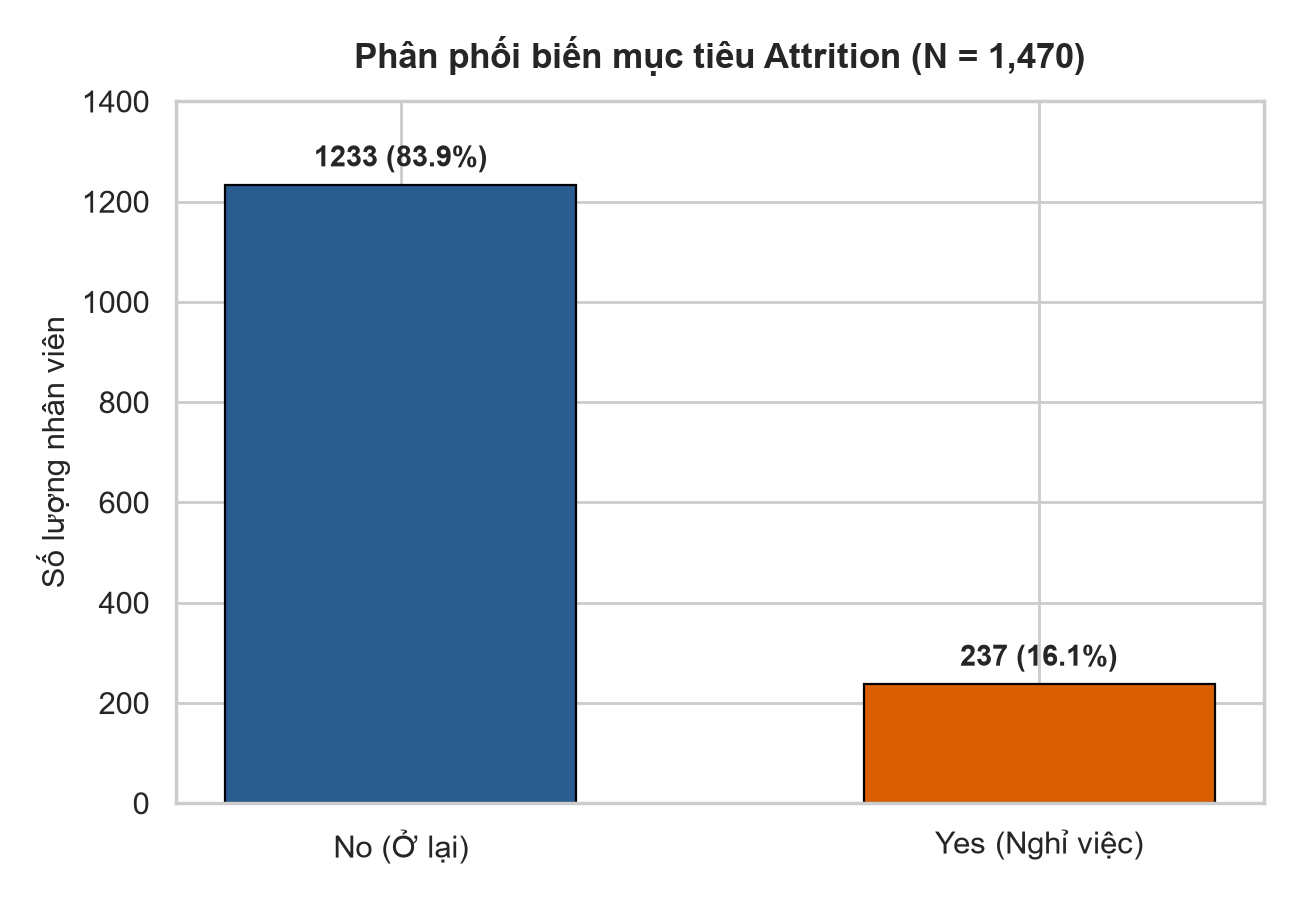
\includegraphics[width=0.68\textwidth]{images/fig1_target_distribution.png}
    \caption{Phân phối biến mục tiêu Attrition trên tập dữ liệu ($N = 1,470$)}
    \label{fig:target_dist}
    \Nguon{Nhóm thực hiện trích xuất từ dữ liệu thực nghiệm}
\end{figure}

Từ Hình~\ref{fig:target_dist}, ta thấy rõ cấu trúc \textbf{mất cân bằng lớp (\textit{Class Imbalance})}:
\begin{itemize}
    \item Nhóm \textbf{\textit{No} (Ở lại)}: gồm $1,233$ nhân viên, chiếm \textbf{83.88\%}.
    \item Nhóm \textbf{\textit{Yes} (Nghỉ việc)}: gồm $237$ nhân viên, chiếm \textbf{16.12\%}.
\end{itemize}
Tỷ lệ giữa lớp đa số và lớp thiểu số là $1233 / 237 \approx \mathbf{5.20 : 1}$. Đặc điểm này dẫn đến hai hệ quả quan trọng cho thiết kế quy trình học máy của nhóm:
\begin{enumerate}
    \item \textbf{Về phương pháp chia dữ liệu}: Bắt buộc phải sử dụng kỹ thuật chia phân tầng (\textit{Stratified Train/Test Split} và \textit{StratifiedKFold}) để đảm bảo tỷ lệ $16.12\%$ mẫu nghỉ việc được giữ nguyên đồng đều trên cả tập huấn luyện và tập kiểm thử.
    \item \textbf{Về độ đo đánh giá (\textit{Evaluation Metrics})}: Một bộ phân loại tầm thường (\textit{Dummy Classifier}) luôn dự đoán mọi nhân viên đều ``Ở lại (\textit{No})'' vẫn sẽ đạt độ chính xác tổng thể $\text{Accuracy} = 83.88\%$, nhưng lại có $\text{Recall} = 0\%$ và $\text{F1-score} = 0\%$ đối với lớp nghỉ việc. Vì vậy, theo đúng yêu cầu của học phần, nhóm không đánh giá mô hình chỉ dựa trên \textit{Accuracy} mà đặt trọng tâm vào \textbf{F1-score}, \textbf{Recall}, \textbf{Precision}, \textbf{Confusion Matrix} và \textbf{ROC-AUC}.
\end{enumerate}

\subsection{Phân tích các đặc trưng số, ngoại lệ (Outliers) và hiện tượng đa cộng tuyến}
Bảng~\ref{tab:thong-ke-mo-ta} trình bày các chỉ số thống kê mô tả của $10$ đặc trưng số tiêu biểu. Tiếp theo, Hình~\ref{fig:boxplots} trực quan hóa phân phối và các điểm ngoại lệ (\textit{outliers}) bằng biểu đồ Boxplot giữa hai lớp \textit{Attrition = No} và \textit{Attrition = Yes}.

\begin{table}[H]
\caption{Thống kê mô tả các đặc trưng số tiêu biểu ($N = 1,470$)}
\label{tab:thong-ke-mo-ta}
\noindent
\begin{tabularx}{\textwidth}{|Y|r|r|r|r|r|r|}
\hline
\textbf{Tên đặc trưng} & \textbf{Mean} & \textbf{Std} & \textbf{Min} & \textbf{Q25} & \textbf{Median} & \textbf{Max} \\
\hline
\textit{Age} (Tuổi) & 36.92 & 9.14 & 18.0 & 30.0 & 36.0 & 60.0 \\
\hline
\textit{MonthlyIncome} (USD) & 6,502.93 & 4,707.96 & 1,009.0 & 2,911.0 & 4,919.0 & 19,999.0 \\
\hline
\textit{TotalWorkingYears} (Năm) & 11.28 & 7.78 & 0.0 & 6.0 & 10.0 & 40.0 \\
\hline
\textit{YearsAtCompany} (Năm) & 7.01 & 6.13 & 0.0 & 3.0 & 5.0 & 40.0 \\
\hline
\textit{YearsInCurrentRole} (Năm) & 4.23 & 3.62 & 0.0 & 2.0 & 3.0 & 18.0 \\
\hline
\textit{YearsSinceLastPromotion} & 2.19 & 3.22 & 0.0 & 0.0 & 1.0 & 15.0 \\
\hline
\textit{DistanceFromHome} (Dặm) & 9.19 & 8.11 & 1.0 & 2.0 & 7.0 & 29.0 \\
\hline
\textit{NumCompaniesWorked} & 2.69 & 2.50 & 0.0 & 1.0 & 2.0 & 9.0 \\
\hline
\textit{PercentSalaryHike} (\%) & 15.21 & 3.66 & 11.0 & 12.0 & 14.0 & 25.0 \\
\hline
\textit{DailyRate} & 802.49 & 403.51 & 102.0 & 465.0 & 802.0 & 1,499.0 \\
\hline
\end{tabularx}
\Nguon{Nhóm thực hiện tính toán từ tập dữ liệu}
\end{table}

\begin{figure}[H]
    \centering
    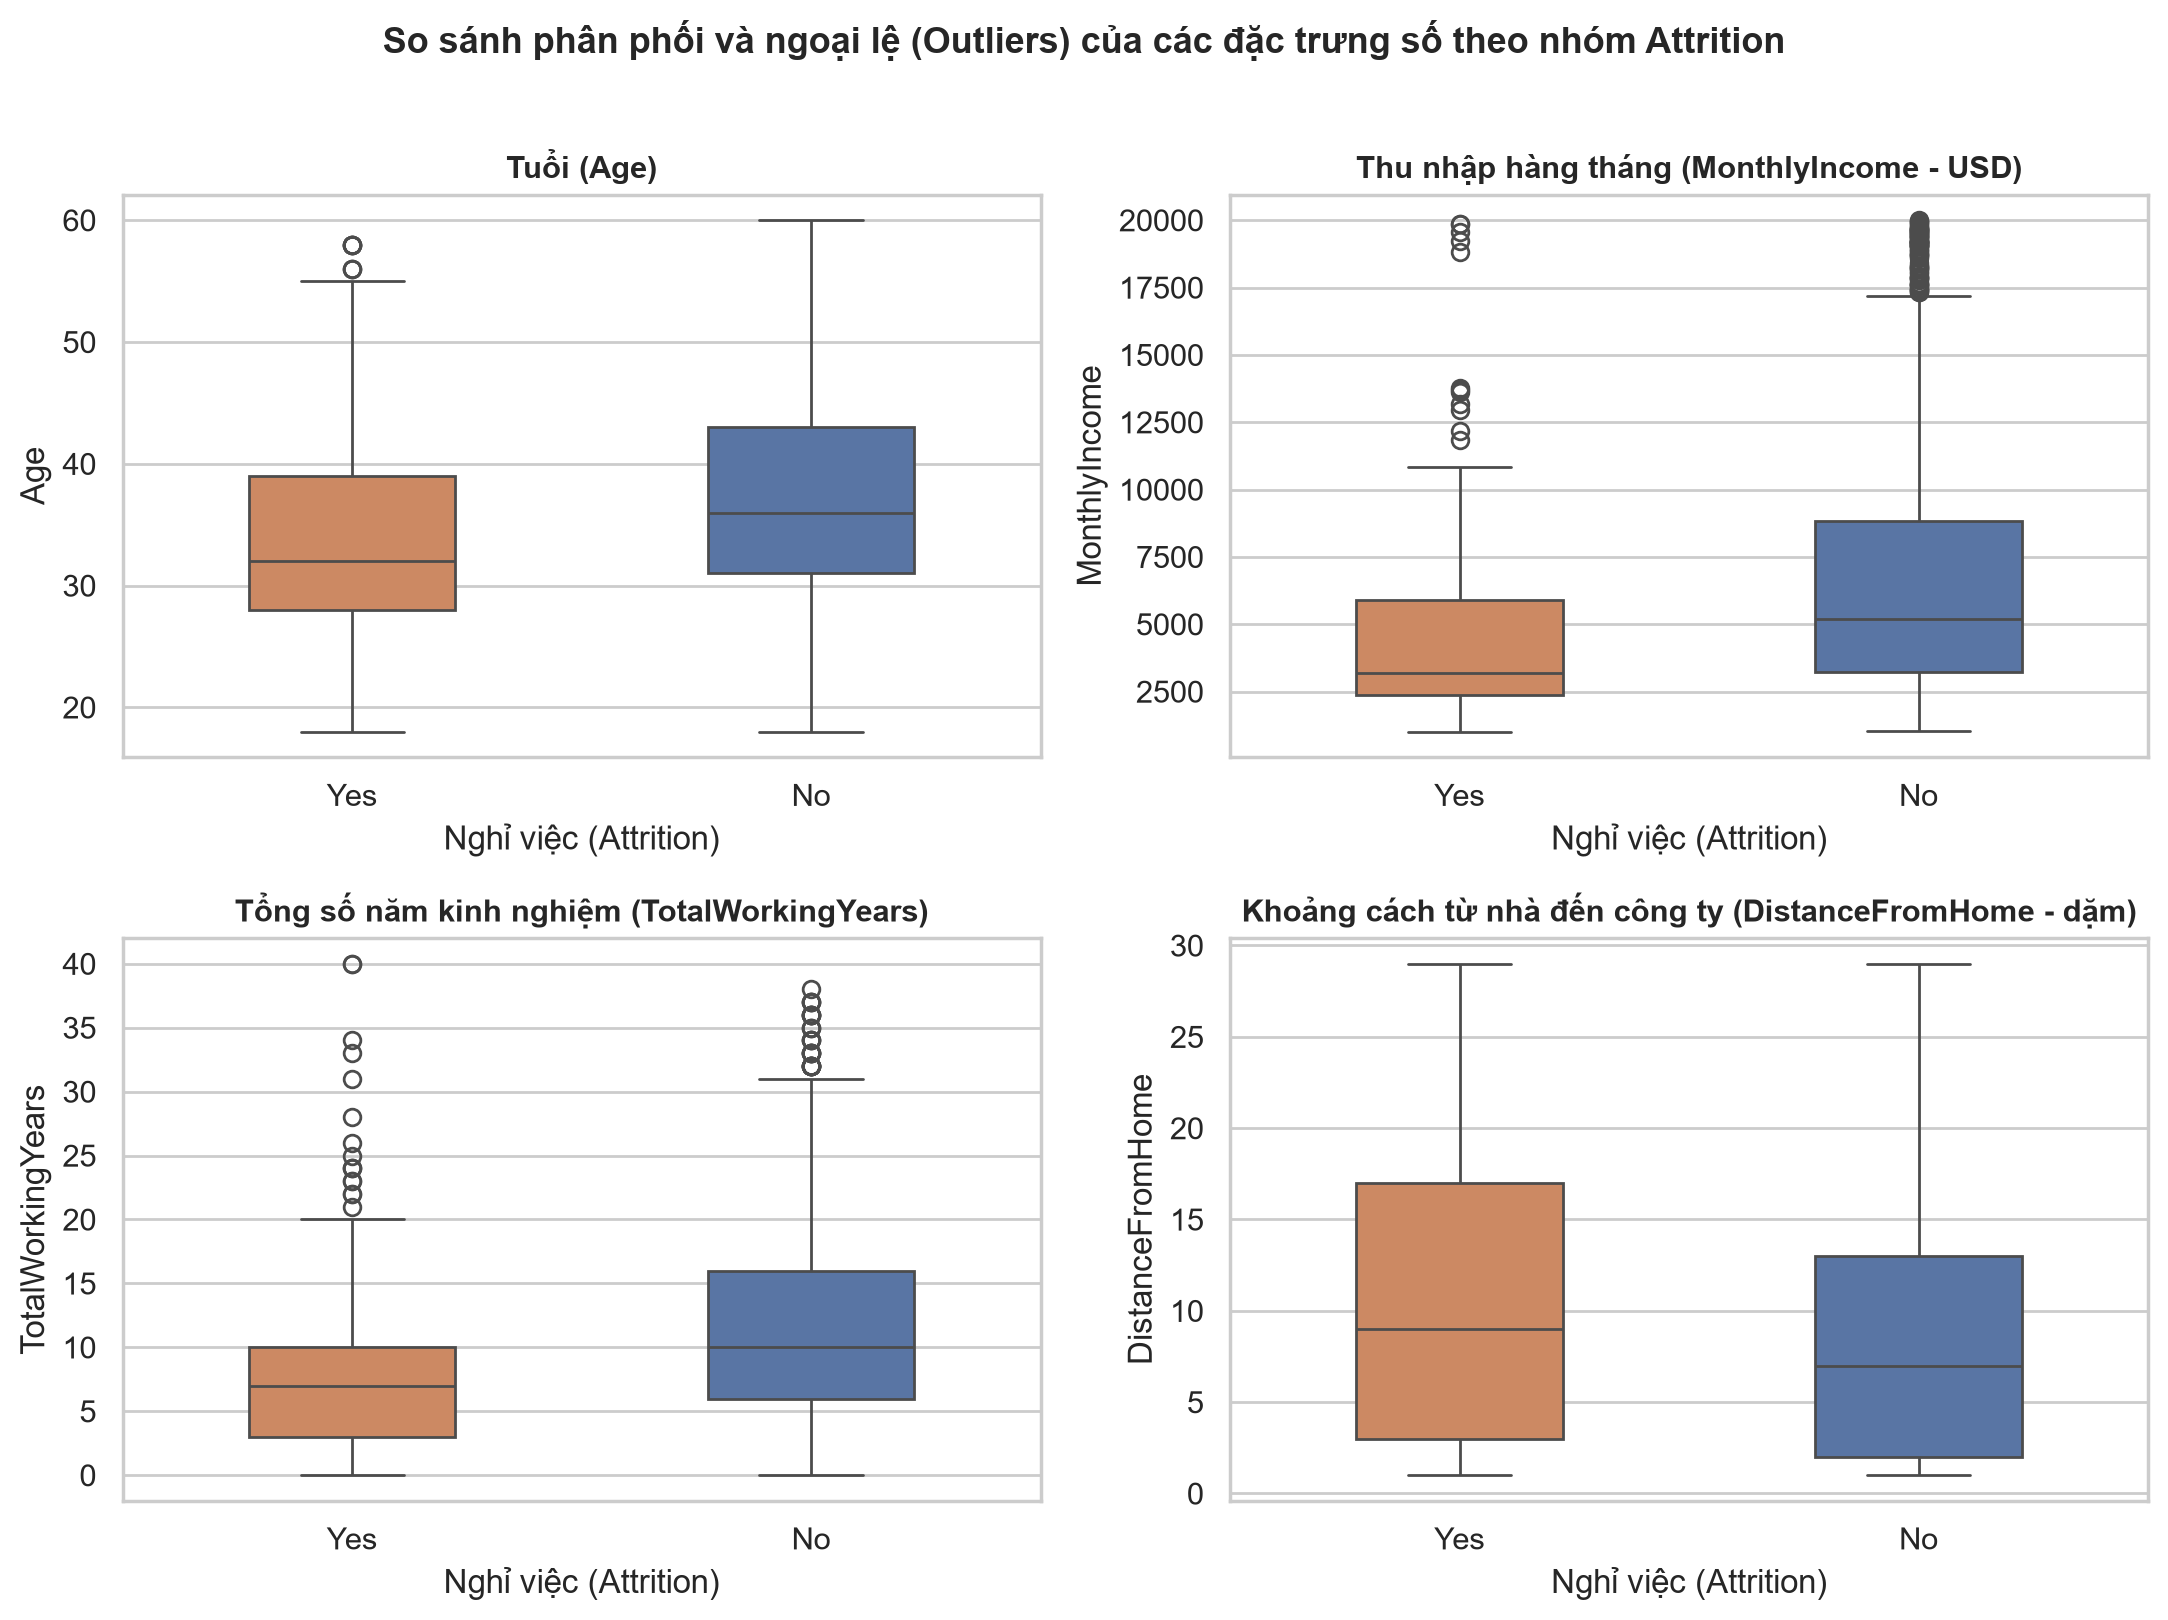
\includegraphics[width=0.95\textwidth]{images/fig2_numerical_boxplots.png}
    \caption{Biểu đồ Boxplot so sánh phân phối và ngoại lệ của các đặc trưng số theo nhóm Attrition}
    \label{fig:boxplots}
    \Nguon{Nhóm thực hiện trích xuất từ dữ liệu thực nghiệm}
\end{figure}

Để kiểm tra mối quan hệ tuyến tính giữa các biến số, Hình~\ref{fig:corr_heatmap} trình bày ma trận tương quan Pearson của các biến số chính và biến mục tiêu đã mã hóa nhị phân \textit{Attrition\_num}.

\begin{figure}[H]
    \centering
    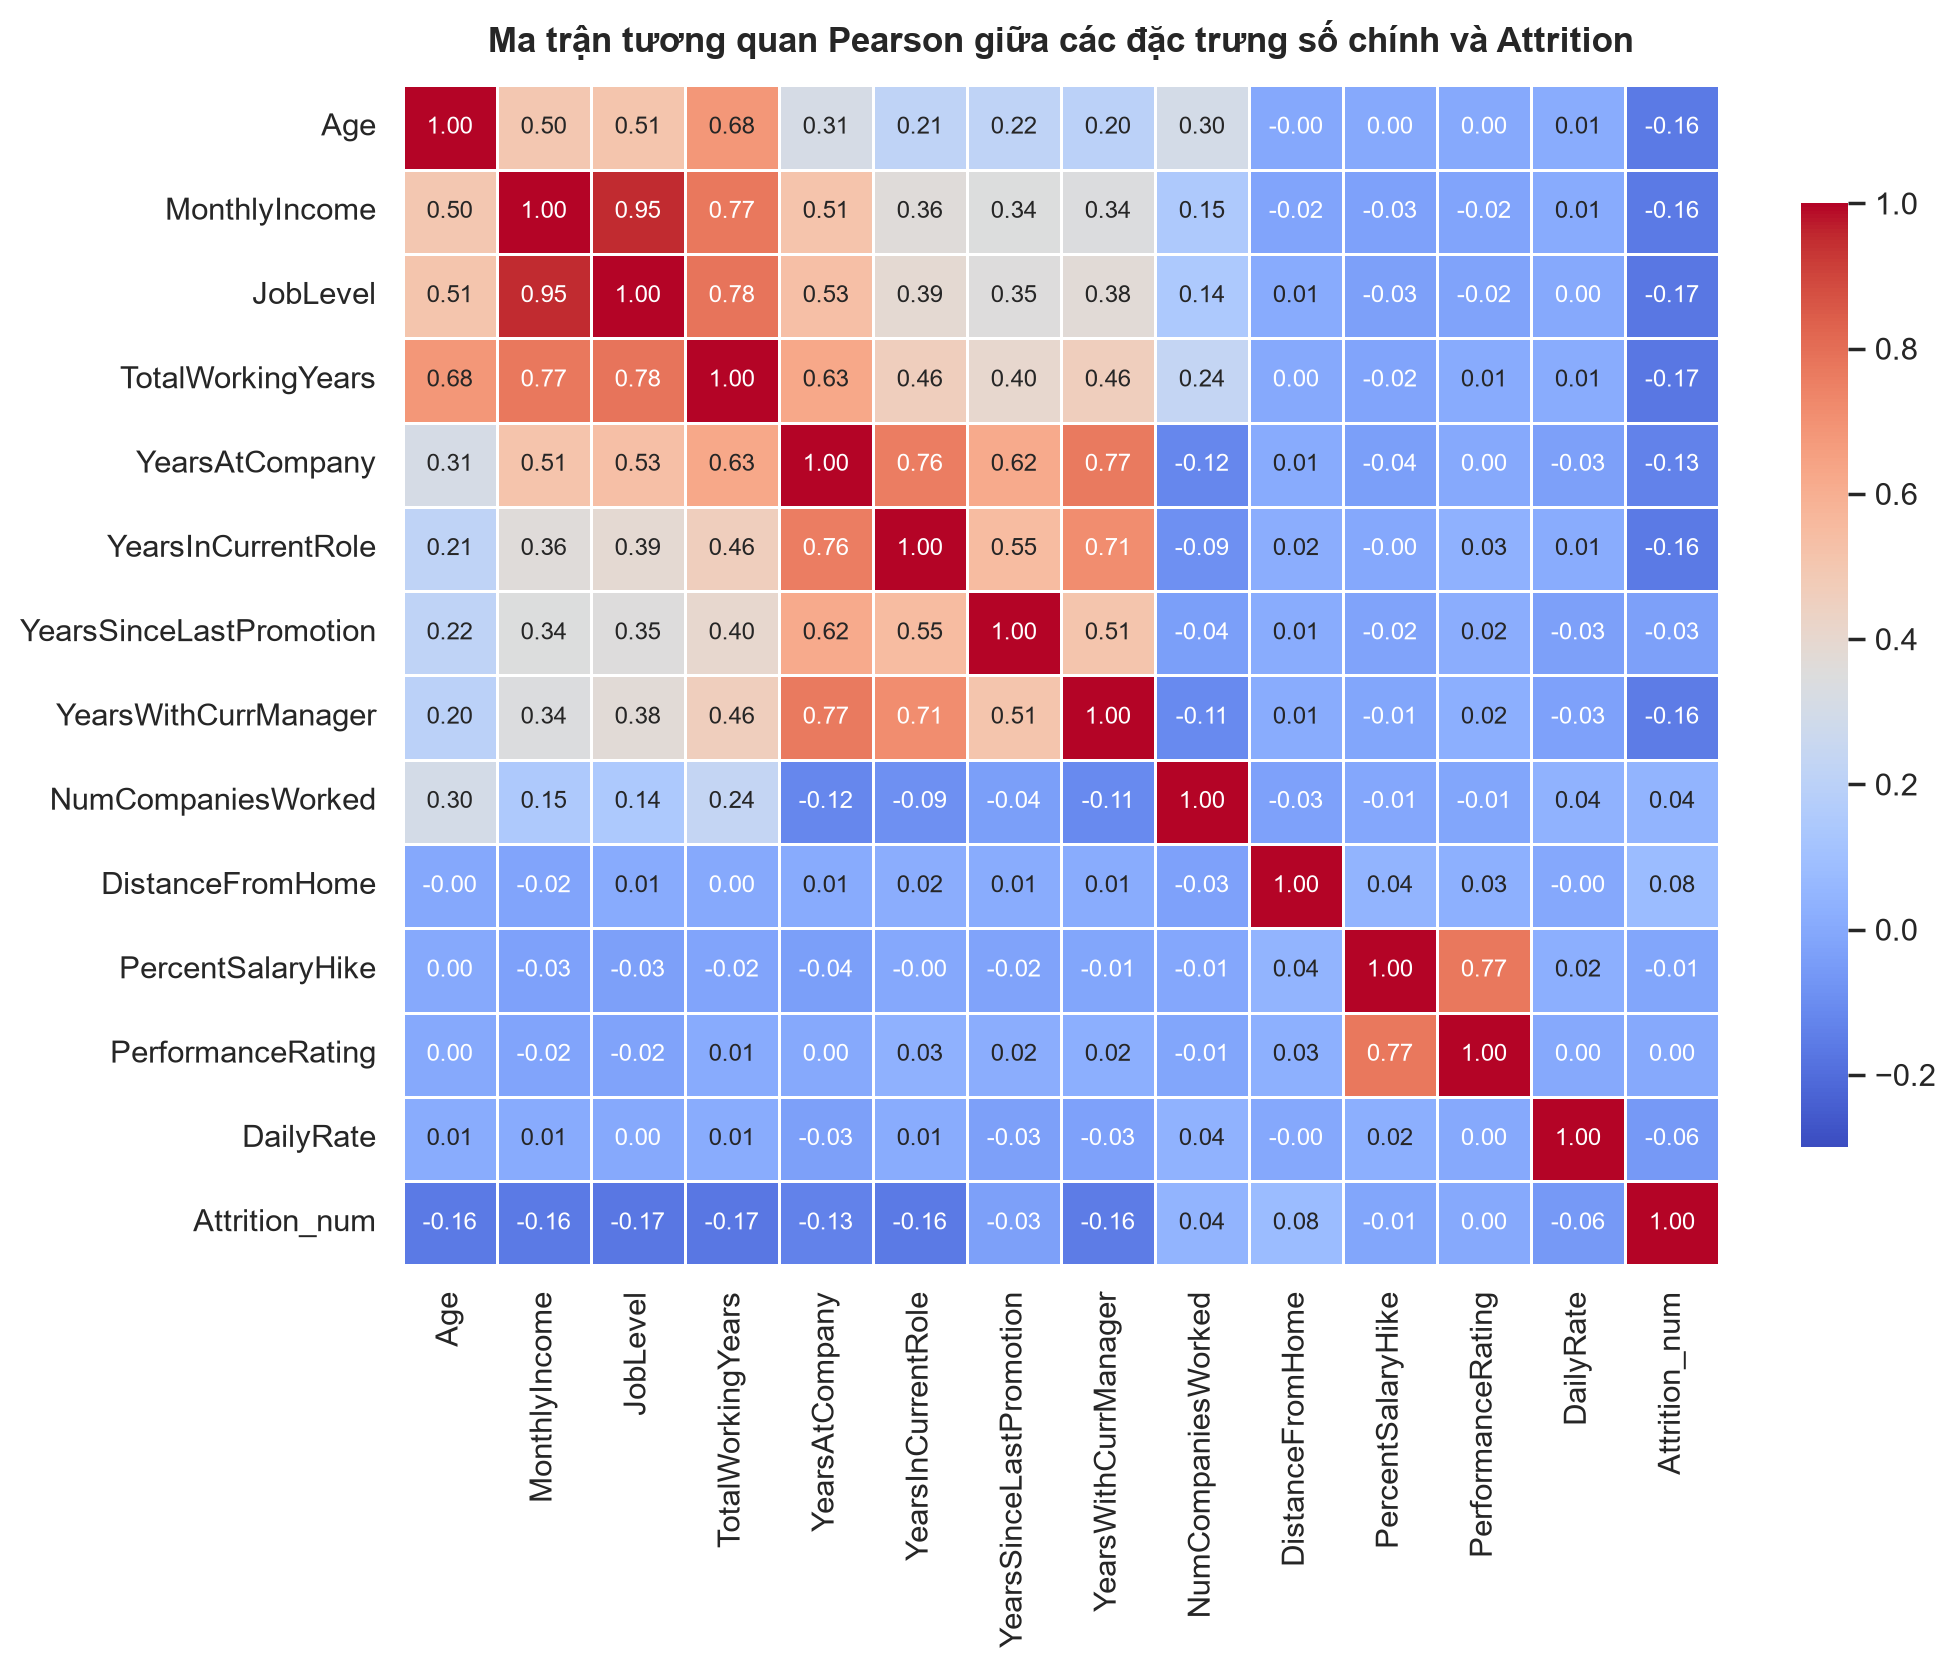
\includegraphics[width=0.88\textwidth]{images/fig4_correlation_heatmap.png}
    \caption{Ma trận tương quan Pearson giữa các đặc trưng số và biến mục tiêu Attrition}
    \label{fig:corr_heatmap}
    \Nguon{Nhóm thực hiện trích xuất từ dữ liệu thực nghiệm}
\end{figure}

Qua đối chiếu Bảng~\ref{tab:thong-ke-mo-ta}, Hình~\ref{fig:boxplots} và Hình~\ref{fig:corr_heatmap}, nhóm rút ra ba nhận định kỹ thuật cốt lõi phục vụ thiết kế Luồng B:
\begin{enumerate}
    \item \textbf{Sự khác biệt rõ rệt về thu nhập, tuổi và thâm niên giữa hai lớp}: Nhóm nhân viên nghỉ việc (\textit{Yes}) có trung vị thu nhập hàng tháng thấp hơn đáng kể so với nhóm ở lại ($\approx 3,202$ USD so với $5,204$ USD; $r = -0.1598$), tổng số năm kinh nghiệm ít hơn ($r = -0.1711$), số năm ở vị trí hiện tại thấp hơn ($r = -0.1605$), tuổi đời trẻ hơn ($r = -0.1592$) và khoảng cách từ nhà đến nơi làm việc xa hơn ($r = +0.0779$).
    \item \textbf{Phân phối lệch phải mạnh và nhiều ngoại lệ (\textit{Outliers})}: Các biến \textit{MonthlyIncome} (trung bình $6,503$ USD nhưng trung vị chỉ $4,919$ USD, cực đại lên tới $19,999$ USD), \textit{TotalWorkingYears} và \textit{YearsAtCompany} có đuôi phân phối lệch phải dài với nhiều điểm ngoại lệ ở nhóm quản lý cấp cao. Nếu chỉ dùng bộ chuẩn hóa \textit{StandardScaler} (chuẩn hóa theo trung bình và độ lệch chuẩn), các ngoại lệ này sẽ kéo dãn thang đo, làm co cụm các nhân viên lương thấp lại gần nhau. Do đó, sử dụng \textbf{\textit{RobustScaler}} (chuẩn hóa theo trung vị và khoảng tứ phân vị IQR) ở Luồng B là giải pháp hợp lý hơn.
    \item \textbf{Phát hiện biến nhiễu ngẫu nhiên và đa cộng tuyến mạnh}:
    \begin{itemize}
        \item Ba biến \textit{DailyRate} ($r = -0.0567$), \textit{HourlyRate} ($r = -0.0068$) và \textit{MonthlyRate} ($r = +0.0152$) có phân phối đều ngẫu nhiên và hoàn toàn không liên quan tới \textit{MonthlyIncome} ($r \approx 0$). Giữ lại $3$ cột này chỉ làm tăng nhiễu khoảng cách Euclidean trong K-NN.
        \item Biến \textit{JobLevel} tương quan gần như tuyệt đối với \textit{MonthlyIncome} ($r = \mathbf{0.95}$); biến \textit{PercentSalaryHike} tương quan chặt với \textit{PerformanceRating} ($r = \mathbf{0.77}$); các biến thâm niên \textit{YearsAtCompany}, \textit{YearsInCurrentRole}, \textit{YearsWithCurrManager} có tương quan lẫn nhau từ $0.71$ đến $0.77$. Hiện tượng \textbf{đa cộng tuyến (\textit{Multicollinearity})} này vi phạm trực tiếp giả định độc lập có điều kiện của thuật toán Naive Bayes, làm nhân đôi trọng số của cùng một nguồn thông tin và gây sai lệch xác suất dự đoán.
    \end{itemize}
\end{enumerate}

\subsection{Phân tích các đặc trưng phân loại và hình thành giả thuyết kỹ thuật đặc trưng}
Hình~\ref{fig:cat_rates} trực quan hóa tỷ lệ nghỉ việc (\%) trên từng giá trị của $4$ thuộc tính phân loại quan trọng nhất: \textit{OverTime}, \textit{MaritalStatus}, \textit{BusinessTravel} và \textit{JobRole}.

\begin{figure}[H]
    \centering
    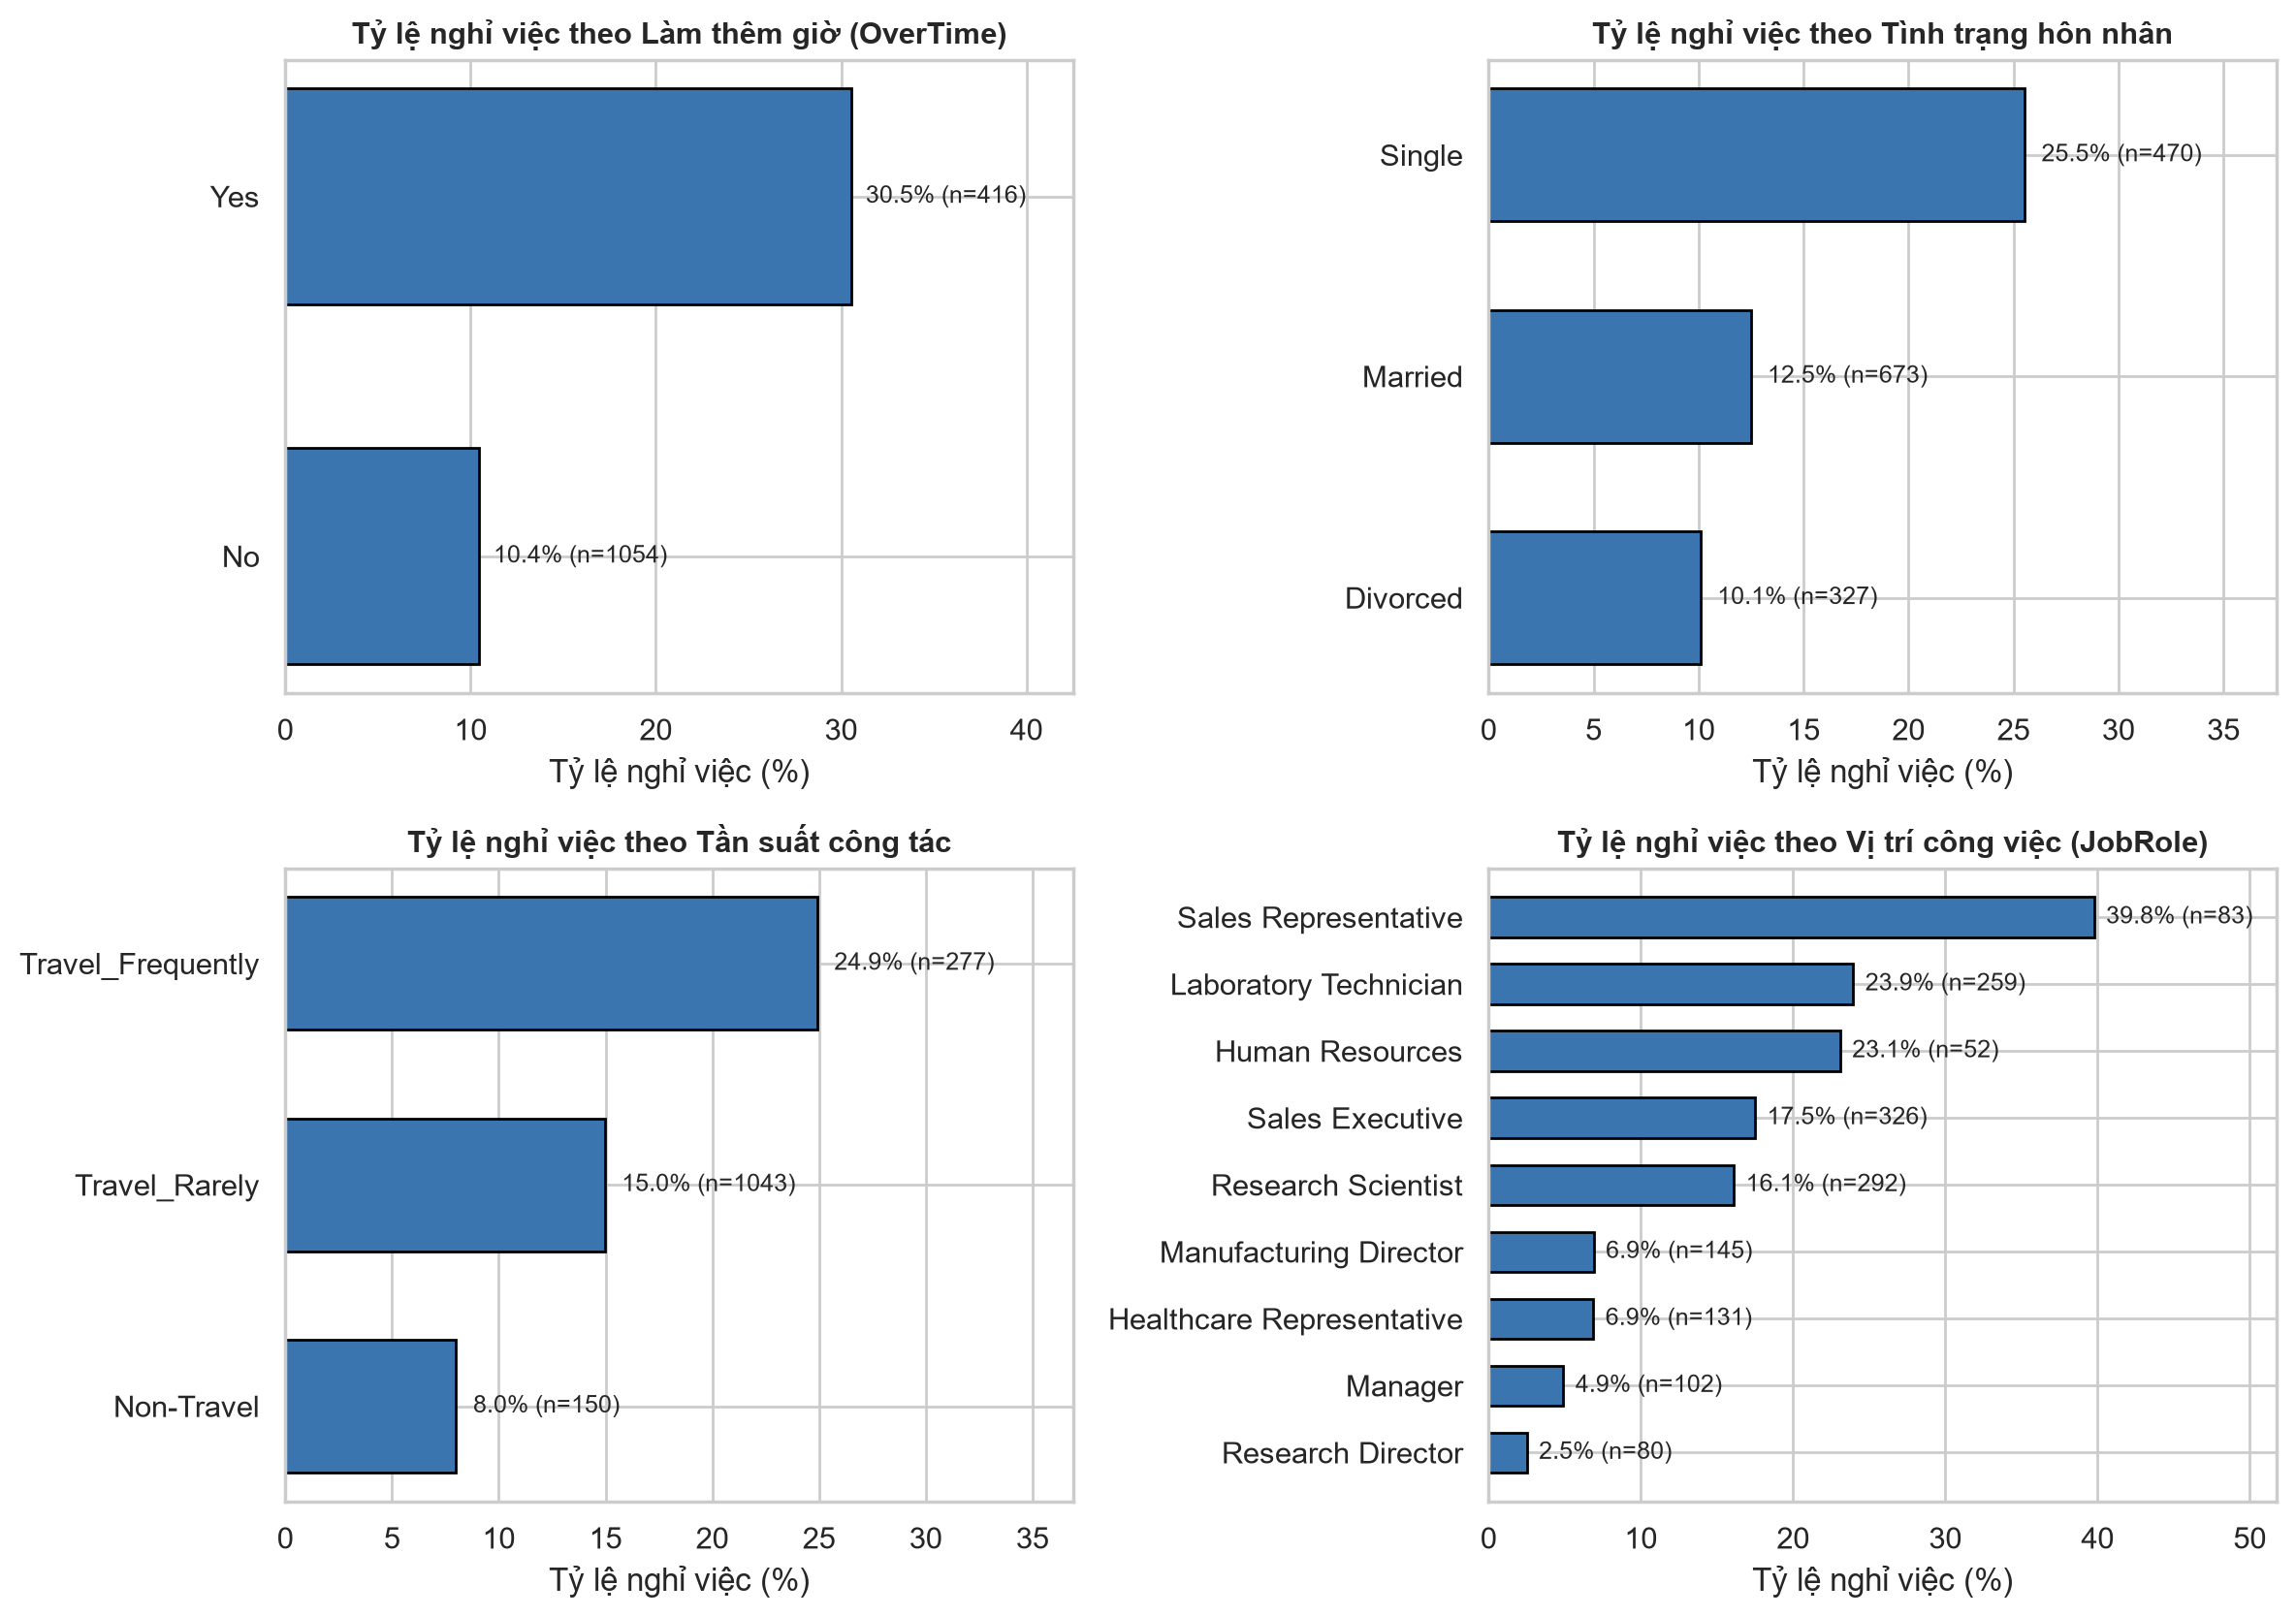
\includegraphics[width=0.96\textwidth]{images/fig3_categorical_rates.png}
    \caption{Tỷ lệ nghỉ việc (\%) theo 4 đặc trưng phân loại quan trọng}
    \label{fig:cat_rates}
    \Nguon{Nhóm thực hiện trích xuất từ dữ liệu thực nghiệm}
\end{figure}

Phân tích thống kê từ Hình~\ref{fig:cat_rates} cho thấy các quy luật nghiệp vụ rất rõ nét:
\begin{itemize}
    \item \textbf{Tác động đột biến của Làm thêm giờ (\textit{OverTime})}: Trong số $416$ nhân viên phải làm thêm giờ (\textit{OverTime = Yes}), có tới $127$ người nghỉ việc (\textbf{30.53\%}), cao gấp gần \textbf{3 lần} so với nhóm không làm thêm giờ (\textbf{10.44\%}, $110/1,054$ người). Đây là biến đơn lẻ có sức phân tách mạnh nhất trong toàn bộ tập dữ liệu.
    \item \textbf{Tình trạng hôn nhân (\textit{MaritalStatus})}: Nhân viên độc thân (\textit{Single}) có tỷ lệ nghỉ việc lên tới \textbf{25.53\%} ($120/470$ người), cao hơn gấp đôi so với nhân viên đã kết hôn (\textit{Married}: \textbf{12.48\%}) và nhân viên đã ly hôn (\textit{Divorced}: \textbf{10.09\%}).
    \item \textbf{Tần suất đi công tác (\textit{BusinessTravel})}: Nhóm phải đi công tác thường xuyên (\textit{Travel\_Frequently}) có tỷ lệ nghỉ việc \textbf{24.91\%}, cao gấp $3$ lần nhóm không phải đi công tác (\textit{Non-Travel}: \textbf{8.00\%}).
    \item \textbf{Vị trí công việc (\textit{JobRole})}: Vị trí nhân viên kinh doanh (\textit{Sales Representative}) có tỷ lệ biến động nhân sự báo động ở mức \textbf{39.76\%} ($33/83$ người), tiếp theo là kỹ thuật viên phòng thí nghiệm (\textit{Laboratory Technician}: \textbf{23.94\%}) và chuyên viên nhân sự (\textit{Human Resources}: \textbf{23.08\%}). Ngược lại, các cấp quản lý như \textit{Research Director} ($2.50\%$) và \textit{Manager} ($4.90\%$) có tỷ lệ nghỉ việc rất thấp.
\end{itemize}

\textbf{Hình thành giả thuyết cho Luồng B}: Nghỉ việc hiếm khi chỉ do một yếu tố đơn lẻ mà thường là kết quả cộng hưởng của nhiều áp lực đồng thời --- chẳng hạn: \textit{nhân viên trẻ/độc thân phải làm thêm giờ liên tục}, \textit{làm thêm giờ kèm theo quãng đường đi làm xa}, hoặc \textit{mức thu nhập thấp không tương xứng với số năm kinh nghiệm và nhiều năm chưa được thăng chức}. Việc tổng hợp các mối quan hệ tương tác này thành các đặc trưng mới sẽ giúp mô hình tuyến tính/xác suất và cây quyết định độ sâu thấp nắm bắt quy luật tốt hơn nhiều so với các cột thô rời rạc.

\chapter[THIẾT KẾ GIẢI PHÁP, QUY TRÌNH HỌC MÁY VÀ PHÂN TÍCH MÃ NGUỒN]{THIẾT KẾ GIẢI PHÁP, QUY TRÌNH HỌC MÁY VÀ PHÂN TÍCH MÃ NGUỒN}

\section{Sơ đồ tổng thể pipeline học máy và chống rò rỉ dữ liệu}

\subsection{Kiến trúc Pipeline học máy tổng quát}
Tuân thủ quy trình thực hiện chung đối với dữ liệu dạng bảng tại Mục 5.1 của Hướng dẫn học phần FIT4013, nhóm thiết kế một pipeline học máy khép kín từ dữ liệu thô đến bước đánh giá và phân tích lỗi, được trình bày tại Sơ đồ~\ref{sodo:pipeline}.

\begin{sodo}[H]
\noindent
\begin{tikzpicture}[
    node distance=0.45cm and 0.45cm,
    box/.style={rectangle, draw=blue!70!black, fill=blue!5, thick, text width=2.75cm, minimum height=1.35cm, align=center, rounded corners=3pt, font=\bfseries\fontsize{13pt}{15pt}\selectfont},
    stream/.style={rectangle, draw=orange!80!black, fill=orange!8, thick, text width=4.35cm, minimum height=1.55cm, align=center, rounded corners=3pt, font=\fontsize{13pt}{15pt}\selectfont},
    arrow/.style={-{Stealth[length=2.2mm]}, thick, draw=gray!80!black}
]
    \node[box] (raw) {Dữ liệu thô\\(1,470 $\times$ 35)};
    \node[box, right=of raw] (split) {Chia 80/20\\Train: 1,176\\Test: 294};
    \node[stream, above right=-0.2cm and 0.45cm of split] (streamA) {\textbf{Luồng A (Cơ bản)}\\Bỏ 4 cột dư + OneHot\\+ \textit{StandardScaler} (44 chiều)};
    \node[stream, below right=-0.2cm and 0.45cm of split] (streamB) {\textbf{Luồng B (Cải tiến)}\\8 đặc trưng HR + \textit{RobustScaler}\\+ \textit{SelectKBest}};
    \node[box, right=5.15cm of split, text width=3.15cm] (models) {Huấn luyện\\1. K-NN\\2. Gaussian NB\\3. Decision Tree\\4. Random Forest};
    \node[box, below=0.55cm of models, text width=3.15cm] (eval) {Đánh giá \& Lỗi\\F1, Recall, AUC\\Confusion Matrix};

    \draw[arrow] (raw) -- (split);
    \draw[arrow] (split.east) -- ++(0.2,0) |- (streamA.west);
    \draw[arrow] (split.east) -- ++(0.2,0) |- (streamB.west);
    \draw[arrow] (streamA.east) -- ++(0.2,0) |- (models.west);
    \draw[arrow] (streamB.east) -- ++(0.2,0) |- (models.west);
    \draw[arrow] (models) -- (eval);
\end{tikzpicture}
\SodoCaption{Kiến trúc Pipeline học máy so sánh Luồng A (Cơ bản) và Luồng B (Cải tiến)}{Nhóm thực hiện tự xây dựng}
\label{sodo:pipeline}
\end{sodo}

\subsection{Chiến lược chia dữ liệu và cơ chế chống rò rỉ dữ liệu (Data Leakage)}
Một trong những yêu cầu bắt buộc quan trọng nhất của học phần là \textit{``Dữ liệu huấn luyện và dữ liệu kiểm thử phải được tách đúng quy trình. Các bước học tham số từ dữ liệu phải được học trên tập huấn luyện để hạn chế data leakage''}. Nhóm đảm bảo nguyên tắc này thông qua ba cơ chế kỹ thuật:
\begin{enumerate}
    \item \textbf{Chia tách phân tầng ngay từ đầu (\textit{Stratified Train/Test Split})}: Trước khi thực hiện bất kỳ phép biến đổi số học nào, toàn bộ $1,470$ bản ghi được chia thành tập Huấn luyện (\textit{X\_train, y\_train}: $1,176$ mẫu, chiếm $80\%$) và tập Kiểm thử độc lập (\textit{X\_test, y\_test}: $294$ mẫu, chiếm $20\%$) với tham số phân tầng \textit{stratify = y} và hạt giống ngẫu nhiên \textit{random\_state = 42}. Nhờ vậy, tập Train chứa $986$ mẫu \textit{No} ($83.84\%$) và $190$ mẫu \textit{Yes} ($16.16\%$); tập Test chứa $247$ mẫu \textit{No} ($84.01\%$) và $47$ mẫu \textit{Yes} ($15.99\%$).
    \item \textbf{Đóng gói toàn bộ biến đổi trong \textit{scikit-learn Pipeline}}: Tất cả các bước tính trung bình và độ lệch chuẩn (\textit{StandardScaler}), trung vị và khoảng tứ phân vị (\textit{RobustScaler}), danh sách nhãn phân loại (\textit{OneHotEncoder}) và điểm thống kê kiểm định $F$-test (\textit{SelectKBest}) đều được đặt bên trong đối tượng \textit{Pipeline}. Khi gọi hàm huấn luyện trên tập \textit{X\_train}, chỉ dữ liệu của $1,176$ mẫu huấn luyện được sử dụng để ước lượng tham số; tập \textit{X\_test} chỉ đi qua phép biến đổi (\textit{transform}) khi dự đoán.
    \item \textbf{Kiểm định chéo phân tầng (\textit{5-Fold Stratified Cross-Validation})}: Khi đánh giá độ ổn định và chọn siêu tham số trên tập Train, mỗi vòng lặp của bộ kiểm định chéo $5$-Fold phân tầng (với \textit{n\_splits = 5}, \textit{shuffle = True}, \textit{random\_state = 42}) tự động khớp lại bộ tiền xử lý trên $4$ fold huấn luyện ($940$ mẫu) và kiểm định trên $1$ fold đánh giá ($236$ mẫu), ngăn chặn hoàn toàn việc rò rỉ thông tin giữa các fold.
\end{enumerate}

\section{Thiết kế hai luồng tiền xử lý và kỹ thuật đặc trưng}

\subsection{Luồng A: Pipeline cơ bản (Baseline Data Preparation)}
Luồng A đóng vai trò là cấu hình xử lý dữ liệu chuẩn mực tối thiểu để làm mốc đối sánh:
\begin{itemize}
    \item \textbf{Xử lý cột dư thừa}: Loại bỏ $3$ cột hằng số (\textit{EmployeeCount}, \textit{Over18}, \textit{StandardHours}) và $1$ cột định danh nhân viên (\textit{EmployeeNumber}).
    \item \textbf{Mã hóa biến phân loại}: Áp dụng bộ mã hóa \textit{OneHotEncoder} (với cấu hình loại bỏ cột đầu tiên \textit{drop = 'first'} và bỏ qua nhãn lạ \textit{handle\_unknown = 'ignore'}) cho $7$ cột chuỗi phân loại (\textit{BusinessTravel}, \textit{Department}, \textit{EducationField}, \textit{Gender}, \textit{JobRole}, \textit{MaritalStatus}, \textit{OverTime}). Tùy chọn \textit{drop = 'first'} giúp loại bỏ sự phụ thuộc tuyến tính hoàn toàn (bẫy biến giả -- \textit{dummy variable trap}) bằng cách biểu diễn một biến phân loại có $C$ nhãn thành $C-1$ cột nhị phân.
    \item \textbf{Chuẩn hóa đặc trưng số}: Áp dụng bộ chuẩn hóa \textit{StandardScaler} đưa $23$ cột số về trung bình $\mu = 0$ và phương sai $\sigma^2 = 1$:
    \[
        z_{ij} = \frac{x_{ij} - \hat{\mu}_j}{\hat{\sigma}_j}
    \]
    Sau khi đi qua bộ biến đổi cột (\textit{ColumnTransformer}) của Luồng A, mỗi mẫu dữ liệu được biểu diễn thành một vector \textbf{44 chiều}.
\end{itemize}

\subsection{Luồng B: Pipeline cải tiến (Domain Feature Engineering \& Robust Preprocessing)}
Khắc phục các hạn chế của dữ liệu thô đã chỉ ra ở Chương 1 (ngoại lệ lệch phải, biến nhiễu ngẫu nhiên, đa cộng tuyến và thiếu các tương tác phi tuyến), Luồng B thực hiện ba cải tiến kỹ thuật đồng bộ:

\subsubsection{1. Tạo 8 đặc trưng nghiệp vụ nhân sự mới (Feature Engineering)}
Bảng~\ref{tab:dac-trung-moi} trình bày công thức toán học, hệ số tương quan với nhãn mục tiêu trên tập Train và ý nghĩa quản trị của $8$ đặc trưng mới do nhóm thiết kế trong lớp \textit{HRFeatureEngineer}.

\begin{table}[H]
\caption{Danh sách 8 đặc trưng mới được tạo trong Luồng B và hệ số tương quan với Attrition}
\label{tab:dac-trung-moi}
\noindent
\begin{tabularx}{\textwidth}{|L{3.5cm}|L{4.8cm}|c|Y|}
\hline
\textbf{Tên đặc trưng mới} & \textbf{Công thức tính toán} & \textbf{Corr ($r$)} & \textbf{Giả thuyết và ý nghĩa HR} \\
\hline
\textit{OverTime\_\allowbreak Single\_Risk} & $\mathbb{I}(\text{OT}=\text{Yes}) \cdot \mathbb{I}(\text{Single})$ & $+0.2951$ & Nhân viên độc thân phải làm thêm giờ có rủi ro nhảy việc cao nhất. \\
\hline
\textit{OverTime\_\allowbreak LowSat\_Risk} & $\mathbb{I}(\text{OT}=\text{Yes}) \cdot \mathbb{I}(\text{TotalSat} \le 2.5)$ & $+0.2651$ & Quá tải giờ làm kết hợp với sự bất mãn về môi trường làm việc. \\
\hline
\textit{JobHoppingRate} & $\text{NumCompanies} / (\text{TotalYears} + 1)$ & $+0.2075$ & Tần suất chuyển việc lịch sử trên mỗi năm đi làm. \\
\hline
\textit{NewHireRisk} & $\mathbb{I}(\text{YearsCty} \le 2 \lor \text{YearsRole} \le 1)$ & $+0.1971$ & Rủi ro sốc văn hóa ở giai đoạn thử việc / mới nhận vị trí. \\
\hline
\textit{TotalSatisfaction} & $(\text{EnvSat} + \text{JobSat} + \text{RelSat} + \text{WLB})/4$ & $-0.1945$ & Chỉ số hài lòng tổng thể, giảm nhiễu phương sai từng câu hỏi lẻ. \\
\hline
\textit{CommuteBurden} & $\text{Distance} \cdot (1 + \mathbb{I}(\text{OT}=\text{Yes}))$ & $+0.1636$ & Gánh nặng đi lại tăng gấp đôi khi nhân viên phải về muộn do tăng ca. \\
\hline
\textit{IncomePer\allowbreak WorkingYear} & $\text{MonthlyIncome} / (\text{TotalYears} + 1)$ & $-0.0725$ & Mức đãi ngộ tương đối trên mỗi năm tích lũy kinh nghiệm. \\
\hline
\textit{StagnationRatio} & $\text{YearsNoPromo} / (\text{YearsCty} + 1)$ & $+0.0445$ & Tỷ lệ thời gian dậm chân tại chỗ chưa được thăng tiến. \\
\hline
\end{tabularx}
\Nguon{Nhóm thực hiện thiết kế và tính toán trên tập huấn luyện ($N_{\text{train}} = 1,176$)}
\end{table}

Đáng chú ý, hai đặc trưng tương tác \textit{OverTime\_Single\_Risk} ($r = +0.2951$) và \textit{OverTime\_LowSat\_Risk} ($r = +0.2651$) đạt hệ số tương quan với \textit{Attrition} cao hơn bất kỳ đặc trưng gốc nào trong bộ dữ liệu (biến gốc mạnh nhất là \textit{TotalWorkingYears} chỉ đạt $|r| = 0.1711$).

\subsubsection{2. Loại bỏ các biến nhiễu và đa cộng tuyến}
Ngoài $4$ cột hằng số/định danh như Luồng A, Luồng B loại bỏ thêm $5$ cột gây hại cho mô hình:
\begin{itemize}
    \item Ba cột tỷ lệ lương ngẫu nhiên \textit{DailyRate}, \textit{HourlyRate}, \textit{MonthlyRate} (có tương quan $\approx 0$ với mục tiêu và làm nhiễu khoảng cách K-NN).
    \item Hai cột đa cộng tuyến mạnh: \textit{JobLevel} (tương quan $r = 0.95$ với \textit{MonthlyIncome}) và \textit{PercentSalaryHike} (tương quan $r = 0.77$ với \textit{PerformanceRating}), giúp giảm hiện tượng nhân trùng lặp bằng chứng trong Gaussian Naive Bayes.
\end{itemize}

\subsubsection{3. Chuẩn hóa kháng ngoại lệ bằng RobustScaler và Chọn lọc đặc trưng}
\begin{itemize}
    \item Thay vì dùng trung bình và độ lệch chuẩn, \textit{RobustScaler} chuẩn hóa các đặc trưng số theo trung vị ($\text{median}$) và khoảng tứ phân vị ($\text{IQR} = Q_{75} - Q_{25}$):
    \[
        x'_{ij} = \frac{x_{ij} - \text{median}(x_j)}{Q_{75}(x_j) - Q_{25}(x_j)}
    \]
    giúp phân phối của \textit{MonthlyIncome} và \textit{IncomePerWorkingYear} không bị bóp méo bởi một số ít Giám đốc có thu nhập gần $20,000$ USD.
    \item Đối với thuật toán dựa trên khoảng cách (K-NN) và rừng ngẫu nhiên, bước chọn lọc đặc trưng \textit{SelectKBest} (sử dụng hàm kiểm định phương sai ANOVA \textit{f\_classif} với $k = 15$) giúp giữ lại đúng $15$ chiều có giá trị thống kê $F$-value cao nhất trên tập Train, loại bỏ hoàn toàn các chiều nhị phân thưa ít thông tin.
\end{itemize}

\section{Mô tả các thuật toán học máy và siêu tham số}

\subsection{Thuật toán K-Nearest Neighbors (K-NN)}
K-NN là thuật toán học lười (\textit{lazy learning}) phi tham số: để dự đoán nhãn của mẫu kiểm thử $\mathbf{x}_*$, thuật toán tìm tập $N_k(\mathbf{x}_*)$ gồm $k$ điểm trong tập huấn luyện có khoảng cách gần $\mathbf{x}_*$ nhất. Nhóm khảo sát hai công thức khoảng cách thuộc họ Minkowski:
\begin{itemize}
    \item \textbf{Khoảng cách Euclidean ($p=2$, mặc định ở Baseline)}: $d_2(\mathbf{u}, \mathbf{v}) = \sqrt{\sum_{j=1}^D (u_j - v_j)^2}$.
    \item \textbf{Khoảng cách Manhattan ($p=1$, ở cấu hình Tuned)}: $d_1(\mathbf{u}, \mathbf{v}) = \sum_{j=1}^D |u_j - v_j|$, vốn ít bị ảnh hưởng bởi các chiều ngoại lệ trong không gian nhiều chiều hơn so với $L_2$.
    \item \textbf{Trọng số biểu quyết (\textit{weights})}: So sánh giữa \textit{uniform} (mỗi láng giềng 1 phiếu bằng nhau) và \textit{distance} (trọng số tỷ lệ nghịch với khoảng cách $w_i = 1 / d(\mathbf{x}_*, \mathbf{x}_i)$, giúp các láng giềng rất gần thuộc lớp thiểu số \textit{Yes} không bị lấn át bởi các điểm lớp \textit{No} ở xa).
\end{itemize}

\subsection{Thuật toán Gaussian Naive Bayes (GNB)}
Gaussian Naive Bayes tính xác suất hậu nghiệm của lớp $c \in \{0, 1\}$ theo định lý Bayes với giả định các đặc trưng độc lập có điều kiện:
\[
    P(y = c \mid \mathbf{x}) \propto P(y = c) \prod_{j=1}^{D} \frac{1}{\sqrt{2\pi \tilde{\sigma}_{jc}^2}} \exp\left( -\frac{(x_j - \mu_{jc})^2}{2\tilde{\sigma}_{jc}^2} \right)
\]
trong đó $\tilde{\sigma}_{jc}^2 = \sigma_{jc}^2 + \varepsilon \cdot \max_{k}(\sigma_k^2)$ là phương sai đã được làm trơn bởi siêu tham số \textbf{\textit{var\_smoothing} ($\varepsilon$)}.
\begin{itemize}
    \item Ở cấu hình mặc định ($\varepsilon = 10^{-9}$), các biến nhị phân hiếm sau One-Hot Encoding (ví dụ \textit{JobRole = Research Director} ở lớp \textit{Yes}) có phương sai $\sigma_{jc}^2 \approx 0$, khiến hàm mật độ xác suất bị cực đoan hóa.
    \item Khi tinh chỉnh $\varepsilon = 0.1$, một lượng phương sai nền đồng nhất được cộng thêm vào mọi đặc trưng, đóng vai trò như phép điều chuẩn (\textit{regularization}) giúp ổn định tỷ số hợp lý (\textit{likelihood ratio}) và giảm mạnh số ca báo động giả (FP).
\end{itemize}

\subsection{Thuật toán Cây quyết định (Decision Tree -- CART) và Mở rộng Random Forest}
\begin{itemize}
    \item \textbf{Decision Tree Classifier}: Xây dựng cây nhị phân bằng cách chọn đặc trưng $j$ và ngưỡng cắt $t$ tại mỗi nút nhằm cực tiểu hóa độ tạp chất Gini có trọng số:
    \[
        G(Q_m) = 1 - \sum_{c \in \{0,1\}} p_{mc}^2
    \]
    Với dữ liệu mất cân bằng $83.9\% : 16.1\%$, cây mặc định (không giới hạn độ sâu \textit{max\_depth = None}) sẽ sinh ra cây rất sâu để học thuộc lòng từng điểm nhiễu nhưng thiên lệch về lớp đa số. Do đó, ở cấu hình Tuned, nhóm sử dụng độ sâu tối đa \textit{max\_depth = 4}, số mẫu tối thiểu tại lá \textit{min\_samples\_leaf = 15} kết hợp cân bằng trọng số lớp \textbf{\textit{class\_weight = 'balanced'}} (tự động gán trọng số lớp $w_c = \frac{N}{2 N_c}$, tức lớp \textit{Yes} có trọng số gấp $\approx 5.2$ lần lớp \textit{No}).
    \item \textbf{Kỹ thuật mở rộng -- Random Forest Classifier}: Kết hợp $200$ cây quyết định độc lập (\textit{n\_estimators = 200}, \textit{max\_depth = 7}, \textit{min\_samples\_leaf = 5}, \textit{class\_weight = 'balanced'}) được huấn luyện trên các mẫu bootstrap và tập con đặc trưng ngẫu nhiên ($\sqrt{D}$), giúp giảm phương sai dự đoán và nâng cao diện tích dưới đường cong ROC-AUC.
\end{itemize}

\section{Phân tích cấu trúc mã nguồn và chức năng các module}

\subsection{Tổ chức thư mục và chức năng từng tệp chương trình}
Bảng~\ref{tab:cau-truc-ma-nguon} mô tả chi tiết cấu trúc các module trong kho mã nguồn của nhóm.

\begin{table}[H]
\caption{Cấu trúc các module mã nguồn và chức năng tương ứng trong dự án}
\label{tab:cau-truc-ma-nguon}
\noindent
\begin{tabularx}{\textwidth}{|L{4.2cm}|L{3.1cm}|Y|}
\hline
\textbf{Đường dẫn tệp / Thư mục} & \textbf{Loại thành phần} & \textbf{Chức năng chính} \\
\hline
\textit{src/pipeline.py} & Module lõi Python & Định nghĩa lớp \textit{HRFeatureEngineer}, hàm chia dữ liệu phân tầng \textit{load\_and\_split\_data} và hàm tạo \textit{Pipeline} cho Luồng A, Luồng B. \\
\hline
\textit{run\_experiments.py} & Script thực nghiệm & Chạy tự động toàn bộ EDA, huấn luyện $13$ cấu hình mô hình, xuất $9$ biểu đồ PNG, lưu mô hình \textit{.pkl} và trích xuất mẫu lỗi FN/FP. \\
\hline
\textit{notebooks/HR\_Employee\_\allowbreak Attrition\_Pipeline.ipynb} & Jupyter Notebook & Trình bày tương tác từng bước phân tích dữ liệu, so sánh Luồng A/B, trực quan hóa kết quả và thảo luận lỗi. \\
\hline
\textit{app.py} & Web App Demo & Ứng dụng giao diện đồ họa cho phép nhập hồ sơ nhân viên, dự đoán xác suất nghỉ việc theo thời gian thực trên cả $4$ mô hình. \\
\hline
\textit{outputs/figures/*.png} & Biểu đồ đầu ra & Lưu trữ $9$ biểu đồ độ phân giải $200$ DPI phục vụ báo cáo và trình chiếu. \\
\hline
\textit{outputs/results/*.csv} & Dữ liệu kết quả & Lưu bảng điểm \textit{experiment\_summary.csv} và danh sách các bản ghi dự đoán sai \textit{error\_analysis\_FN/FP.csv}. \\
\hline
\textit{README.md, requirements.txt, AI\_USAGE.md} & Tài liệu tái lập & Hướng dẫn cài đặt môi trường, lệnh chạy tái tạo kết quả và khai báo liêm chính học thuật về sử dụng AI. \\
\hline
\end{tabularx}
\Nguon{Nhóm thực hiện tổng hợp}
\end{table}

\subsection{Phân tích đoạn mã nguồn cốt lõi xây dựng Pipeline Luồng A và Luồng B}
Đoạn mã dưới đây trích từ tệp \textit{src/pipeline.py}, minh họa cách nhóm cài đặt lớp \textit{HRFeatureEngineer} và đóng gói thành \textit{Pipeline} chuẩn mực không gây rò rỉ dữ liệu:

\begin{lstlisting}[caption={Định nghĩa lớp HRFeatureEngineer và hàm khởi tạo Luồng B trong src/pipeline.py}]
class HRFeatureEngineer(BaseEstimator, TransformerMixin):
    def __init__(self, drop_noisy=True):
        self.drop_noisy = drop_noisy

    def fit(self, X, y=None):
        return self

    def transform(self, X):
        X = X.copy()
        X['TotalSatisfaction'] = (
            X['EnvironmentSatisfaction'] + X['JobSatisfaction'] +
            X['RelationshipSatisfaction'] + X['WorkLifeBalance']
        ) / 4.0
        X['IncomePerWorkingYear'] = X['MonthlyIncome'] / (X['TotalWorkingYears'] + 1.0)
        X['StagnationRatio'] = X['YearsSinceLastPromotion'] / (X['YearsAtCompany'] + 1.0)
        X['JobHoppingRate'] = X['NumCompaniesWorked'] / (X['TotalWorkingYears'] + 1.0)
        X['NewHireRisk'] = (
            (X['YearsAtCompany'] <= 2) | (X['YearsInCurrentRole'] <= 1)
        ).astype(int)

        ot_bin = (X['OverTime'] == 'Yes').astype(int)
        single_bin = (X['MaritalStatus'] == 'Single').astype(int)
        X['OverTime_Single_Risk'] = ot_bin * single_bin
        X['OverTime_LowSat_Risk'] = ot_bin * (X['TotalSatisfaction'] <= 2.5).astype(int)
        X['CommuteBurden'] = X['DistanceFromHome'] * (1 + ot_bin)

        cols_to_drop = list(DROP_COLS_BASIC)
        if self.drop_noisy:
            cols_to_drop += [
                'DailyRate', 'HourlyRate', 'MonthlyRate',
                'JobLevel', 'PercentSalaryHike'
            ]
        return X.drop(columns=[c for c in cols_to_drop if c in X.columns])
\end{lstlisting}

\chapter[THỬ NGHIỆM, ĐÁNH GIÁ KẾT QUẢ, THẢO LUẬN VÀ PHÂN TÍCH LỖI]{THỬ NGHIỆM, ĐÁNH GIÁ KẾT QUẢ, THẢO LUẬN VÀ PHÂN TÍCH LỖI}

\section{Thiết lập thí nghiệm và các độ đo đánh giá}

\subsection{Môi trường thực nghiệm và thiết lập tham số tái lập}
Toàn bộ các thí nghiệm được thực thi tự động thông qua tệp \textit{run\_experiments.py} với các tham số cố định nhằm đảm bảo khả năng tái tạo tuyệt đối (\textit{100\% Reproducibility}):
\begin{itemize}
    \item \textbf{Hạt giống ngẫu nhiên (\textit{random\_state})}: Cố định \textit{RANDOM\_STATE = 42} cho mọi bước chia dữ liệu, kiểm định chéo $5$-Fold phân tầng và khởi tạo thuật toán (\textit{DecisionTreeClassifier}, \textit{RandomForestClassifier}).
    \item \textbf{Kích thước mẫu}: Tập Huấn luyện có $N_{\text{train}} = 1,176$ mẫu ($986$ \textit{No}, $190$ \textit{Yes}); tập Kiểm thử có $N_{\text{test}} = 294$ mẫu ($247$ \textit{No}, $47$ \textit{Yes}).
    \item \textbf{Phương án Baseline}: Với mỗi thuật toán trong $3$ thuật toán cốt lõi (K-NN, Gaussian NB, Decision Tree), cấu hình mặc định của thư viện \textit{scikit-learn} chạy trên \textbf{Luồng A (Pipeline cơ bản)} được dùng làm mốc Baseline chuẩn để định lượng mức độ cải thiện.
\end{itemize}

\subsection{Hệ thống các độ đo đánh giá cho dữ liệu mất cân bằng}
Gọi $\text{TP}$ (True Positive) là số nhân viên nghỉ việc được dự đoán đúng là nghỉ việc, $\text{TN}$ (True Negative) là số nhân viên ở lại được dự đoán đúng là ở lại, $\text{FP}$ (False Positive -- Báo động giả) là số nhân viên ở lại bị dự đoán nhầm là nghỉ việc, và $\text{FN}$ (False Negative -- Bỏ sót) là số nhân viên thực tế nghỉ việc nhưng mô hình dự đoán ở lại. Nhóm sử dụng $5$ chỉ số đánh giá chính:
\begin{enumerate}
    \item \textbf{Accuracy}: $\dfrac{\text{TP} + \text{TN}}{\text{TP} + \text{TN} + \text{FP} + \text{FN}}$ --- Độ chính xác toàn cục (chỉ mang tính tham khảo do lớp \textit{No} chiếm $84\%$).
    \item \textbf{Precision (Lớp \textit{Yes})}: $\dfrac{\text{TP}}{\text{TP} + \text{FP}}$ --- Trong số những nhân viên được mô hình cảnh báo sắp nghỉ việc, bao nhiêu phần trăm thực sự nghỉ việc.
    \item \textbf{Recall / Độ nhạy (Lớp \textit{Yes})}: $\dfrac{\text{TP}}{\text{TP} + \text{FN}}$ --- Trong tổng số $47$ nhân viên thực sự nghỉ việc trên tập Test, mô hình phát hiện được bao nhiêu phần trăm. Đây là chỉ số sống còn để không bỏ sót nhân tài rời bỏ công ty.
    \item \textbf{F1-score (Lớp \textit{Yes})}: $\dfrac{2 \times \text{Precision} \times \text{Recall}}{\text{Precision} + \text{Recall}}$ --- Trung bình điều hòa cân bằng giữa Precision và Recall, được nhóm chọn làm \textbf{độ đo chính để xếp hạng mô hình}.
    \item \textbf{ROC-AUC}: Diện tích dưới đường cong ROC, đo lường khả năng phân tách xác suất giữa hai lớp trên mọi ngưỡng cắt quyết định $\tau \in (0, 1)$.
\end{enumerate}

\section{Kết quả thực nghiệm và trực quan hóa}

\subsection{Bảng tổng hợp kết quả thực nghiệm toàn diện}
Bảng~\ref{tab:ket-qua-thuc-nghiem} trình bày chi tiết kết quả của toàn bộ $13$ phương án thử nghiệm trên cả kiểm định chéo $5$-Fold CV (trên tập Train) và trên tập Kiểm thử độc lập ($N_{\text{test}} = 294$).

\begin{table}[H]
\caption{Bảng tổng hợp kết quả so sánh giữa Luồng A, Luồng B và các cấu hình mô hình ($N_{\text{test}} = 294$)}
\label{tab:ket-qua-thuc-nghiem}
\noindent
\setlength{\tabcolsep}{3.5pt}
\begin{tabularx}{\textwidth}{|L{1.8cm}|Y|c|c|c|c|c|c|c|c|}
\hline
\textbf{Luồng} & \textbf{Mô hình và cấu hình} & \textbf{CV F1} & \textbf{Acc} & \textbf{Prec} & \textbf{Rec} & \textbf{F1} & \textbf{AUC} & \textbf{TP/FN} & \textbf{FP/TN} \\
\hline
Luồng A & K-NN (Baseline, $k=5$)        & 0.226 & 0.837 & 0.455 & 0.106 & 0.172 & 0.618 & 5 / 42  & 6 / 241  \\
\hline
Luồng A & K-NN (Tuned, $k=11$)          & 0.193 & 0.840 & 0.500 & 0.064 & 0.113 & 0.692 & 3 / 44  & 3 / 244  \\
\hline
Luồng A & Gaussian NB ($10^{-9}$)       & 0.390 & 0.616 & 0.250 & \textbf{0.702} & 0.369 & 0.696 & 33 / 14 & 99 / 148 \\
\hline
Luồng A & Gaussian NB (sm=0.1)          & 0.475 & 0.745 & 0.329 & 0.575 & 0.419 & 0.732 & 27 / 20 & 55 / 192 \\
\hline
Luồng A & Decision Tree (Baseline)      & 0.371 & 0.759 & 0.293 & 0.362 & 0.324 & 0.598 & 17 / 30 & 41 / 206 \\
\hline
Luồng A & Decision Tree (Tuned, d=4)    & 0.422 & 0.701 & 0.270 & 0.511 & 0.353 & 0.696 & 24 / 23 & 65 / 182 \\
\hline
Luồng B & K-NN (Baseline, $k=5$)        & 0.365 & 0.833 & 0.438 & 0.149 & 0.222 & 0.660 & 7 / 40  & 9 / 238  \\
\hline
Luồng B & K-NN (Tuned, $k=7$)           & 0.318 & 0.850 & \textbf{0.600} & 0.192 & 0.290 & 0.698 & 9 / 38  & 6 / 241  \\
\hline
Luồng B & Gaussian NB ($10^{-9}$)       & 0.487 & 0.803 & 0.425 & 0.660 & 0.517 & \textbf{0.770} & 31 / 16 & 42 / 205 \\
\hline
\textbf{Luồng B} & \textbf{Gaussian NB (sm=0.1)} & \textbf{0.541} & \textbf{0.857} & 0.549 & 0.596 & \textbf{0.571} & 0.769 & \textbf{28 / 19} & \textbf{23 / 224} \\
\hline
Luồng B & Decision Tree (Baseline)      & 0.344 & 0.759 & 0.260 & 0.277 & 0.268 & 0.563 & 13 / 34 & 37 / 210 \\
\hline
Luồng B & Decision Tree (Tuned, d=4)    & 0.409 & 0.752 & 0.333 & 0.553 & 0.416 & 0.703 & 26 / 21 & 52 / 195 \\
\hline
Mở rộng & Random Forest (200 cây)       & 0.503 & 0.765 & 0.355 & 0.575 & 0.439 & 0.761 & 27 / 20 & 49 / 198 \\
\hline
\end{tabularx}
\Nguon{Nhóm thực hiện tổng hợp từ tệp kết quả experiment\_summary.csv}
\end{table}

\subsection{So sánh hiệu quả giữa Luồng A (Cơ bản) và Luồng B (Cải tiến)}
Hình~\ref{fig:stream_comp} trực quan hóa mức tăng trưởng về \textit{F1-score} và \textit{ROC-AUC} khi chuyển từ Luồng A sang Luồng B trên cả ba thuật toán đã tinh chỉnh.

\begin{figure}[H]
    \centering
    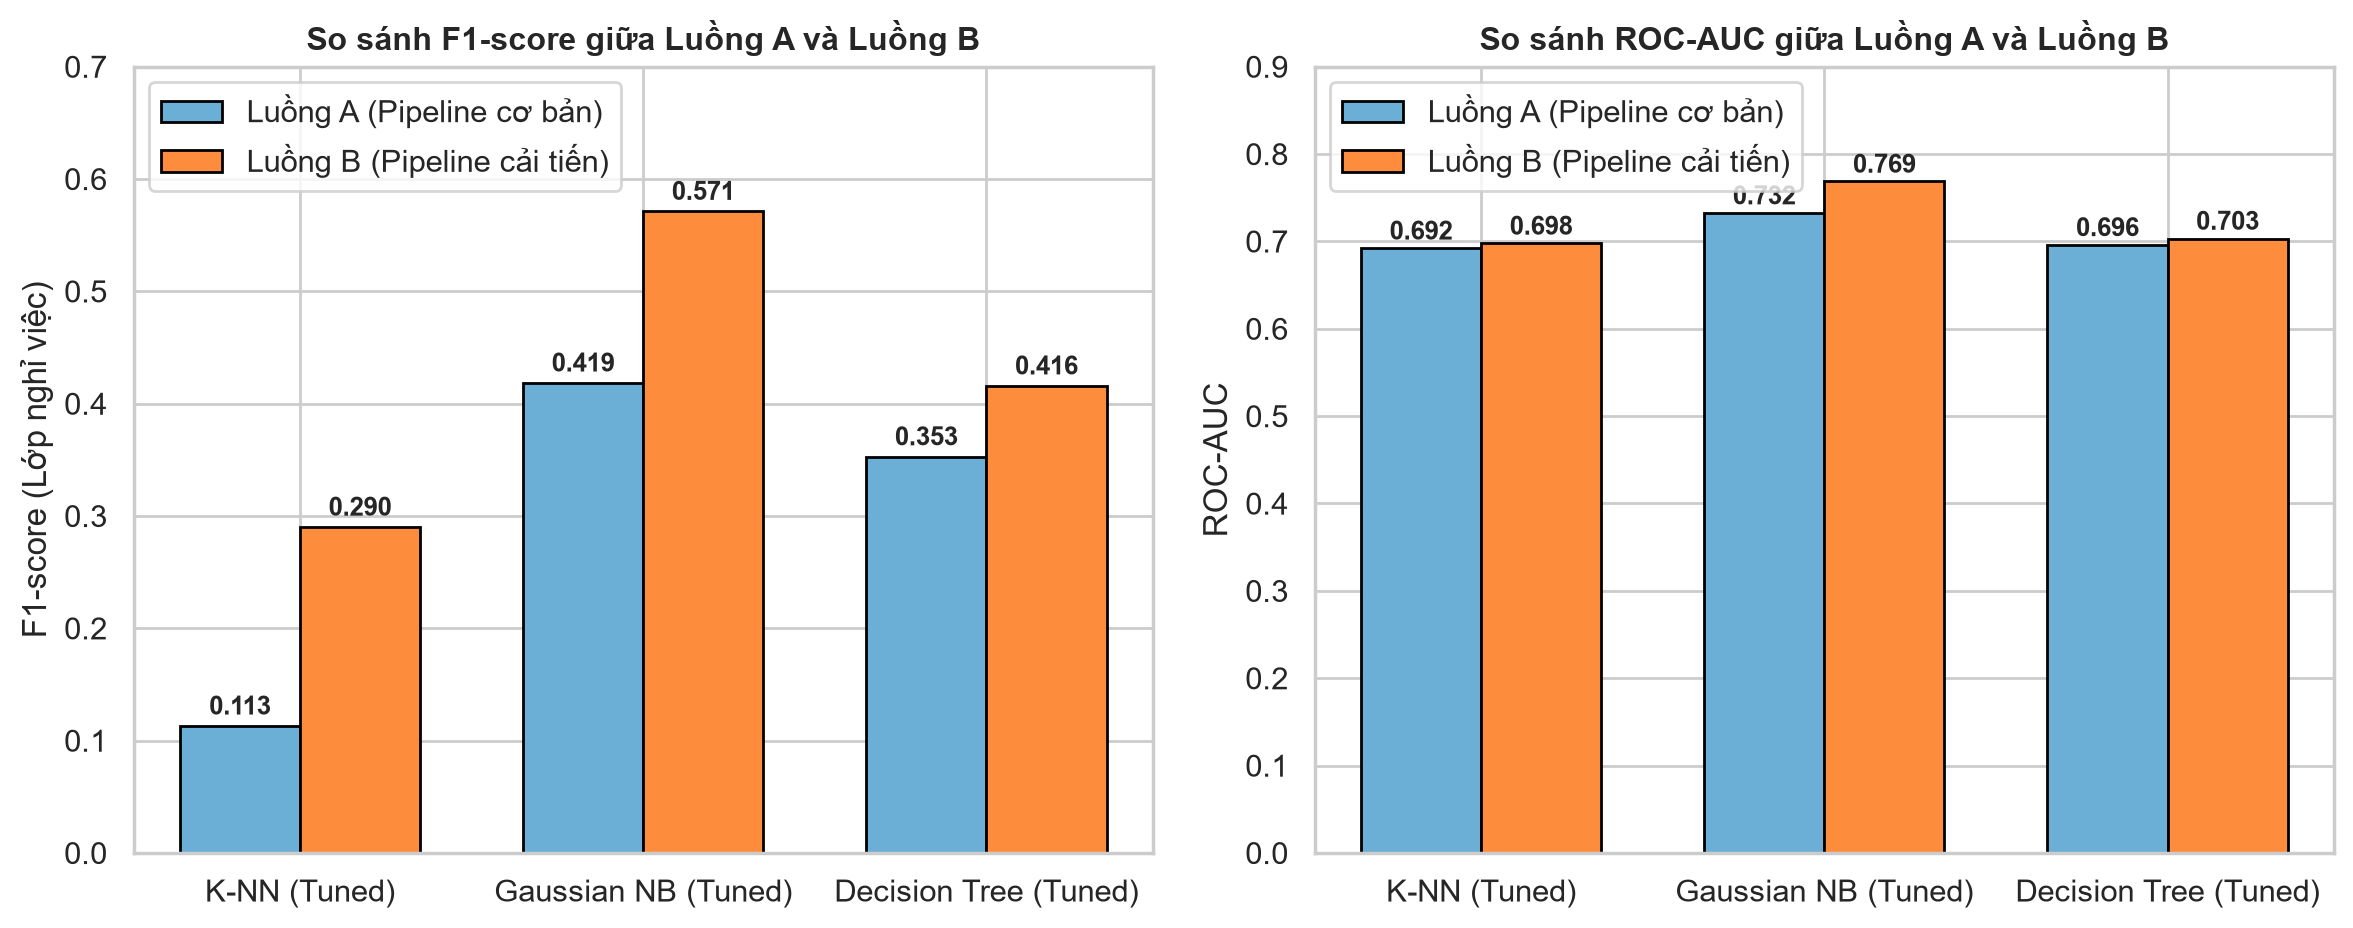
\includegraphics[width=0.95\textwidth]{images/fig6_stream_comparison.png}
    \caption{So sánh chỉ số F1-score và ROC-AUC giữa Luồng A (Cơ bản) và Luồng B (Cải tiến)}
    \label{fig:stream_comp}
    \Nguon{Nhóm thực hiện trích xuất từ dữ liệu thực nghiệm}
\end{figure}

Số liệu thực nghiệm tại Bảng~\ref{tab:ket-qua-thuc-nghiem} và Hình~\ref{fig:stream_comp} khẳng định giả thuyết của nhóm là hoàn toàn chính xác: \textbf{Luồng B cải thiện đồng loạt hiệu quả của cả ba thuật toán}:
\begin{itemize}
    \item \textbf{Đối với K-NN (Tuned)}: Trên Luồng A ($44$ chiều), K-NN bị nhiễu nặng bởi các biến tỷ lệ lương ngẫu nhiên và các biến nhị phân thưa, chỉ đạt $\text{F1} = 0.1132$ ($\text{TP} = 3$ ca). Khi sang Luồng B kết hợp \textit{RobustScaler} và chọn lọc $15$ đặc trưng bằng \textit{SelectKBest}, số ca phát hiện đúng tăng gấp $3$ lần ($\text{TP} = 9$), kéo \textit{F1-score} tăng lên \textbf{0.2903} (\textbf{+156.4\%}) và \textit{Precision} đạt mức cao nhất \textbf{60.00\%}.
    \item \textbf{Đối với Decision Tree (Tuned)}: Trên Luồng A, cây quyết định độ sâu $4$ đạt $\text{F1} = 0.3529$ ($\text{Recall} = 51.06\%, \text{FP} = 65$). Trên Luồng B, nhờ các đặc trưng tổng hợp như \textit{OverTime\_Single\_Risk} và \textit{TotalSatisfaction}, cây quyết định chỉ cần $4$ tầng phân nhánh đã đạt $\text{F1} = \mathbf{0.4160}$ (\textbf{+17.9\%}), nâng \textit{Recall} lên \textbf{55.32\%} đồng thời giảm báo động giả từ $65$ xuống $52$ ca.
    \item \textbf{Đối với Gaussian Naive Bayes (Tuned)}: Đây là mô hình hưởng lợi lớn nhất từ Luồng B. Nhờ loại bỏ các biến đa cộng tuyến và bổ sung các đặc trưng tương tác, \textit{F1-score} trên tập Test tăng vọt từ $0.4186$ lên \textbf{0.5714} (\textbf{+36.5\%}), \textit{Accuracy} tăng từ $74.49\%$ lên \textbf{85.71\%}, và \textit{ROC-AUC} kiểm định chéo $5$-Fold đạt tới \textbf{0.8007}.
\end{itemize}

\subsection{Phân tích ảnh hưởng của siêu tham số (Hyperparameter Sensitivity)}
Hình~\ref{fig:hyper_tuning} biểu diễn sự biến thiên hiệu năng của ba thuật toán khi thay đổi các siêu tham số cốt lõi trên Luồng B.

\begin{figure}[H]
    \centering
    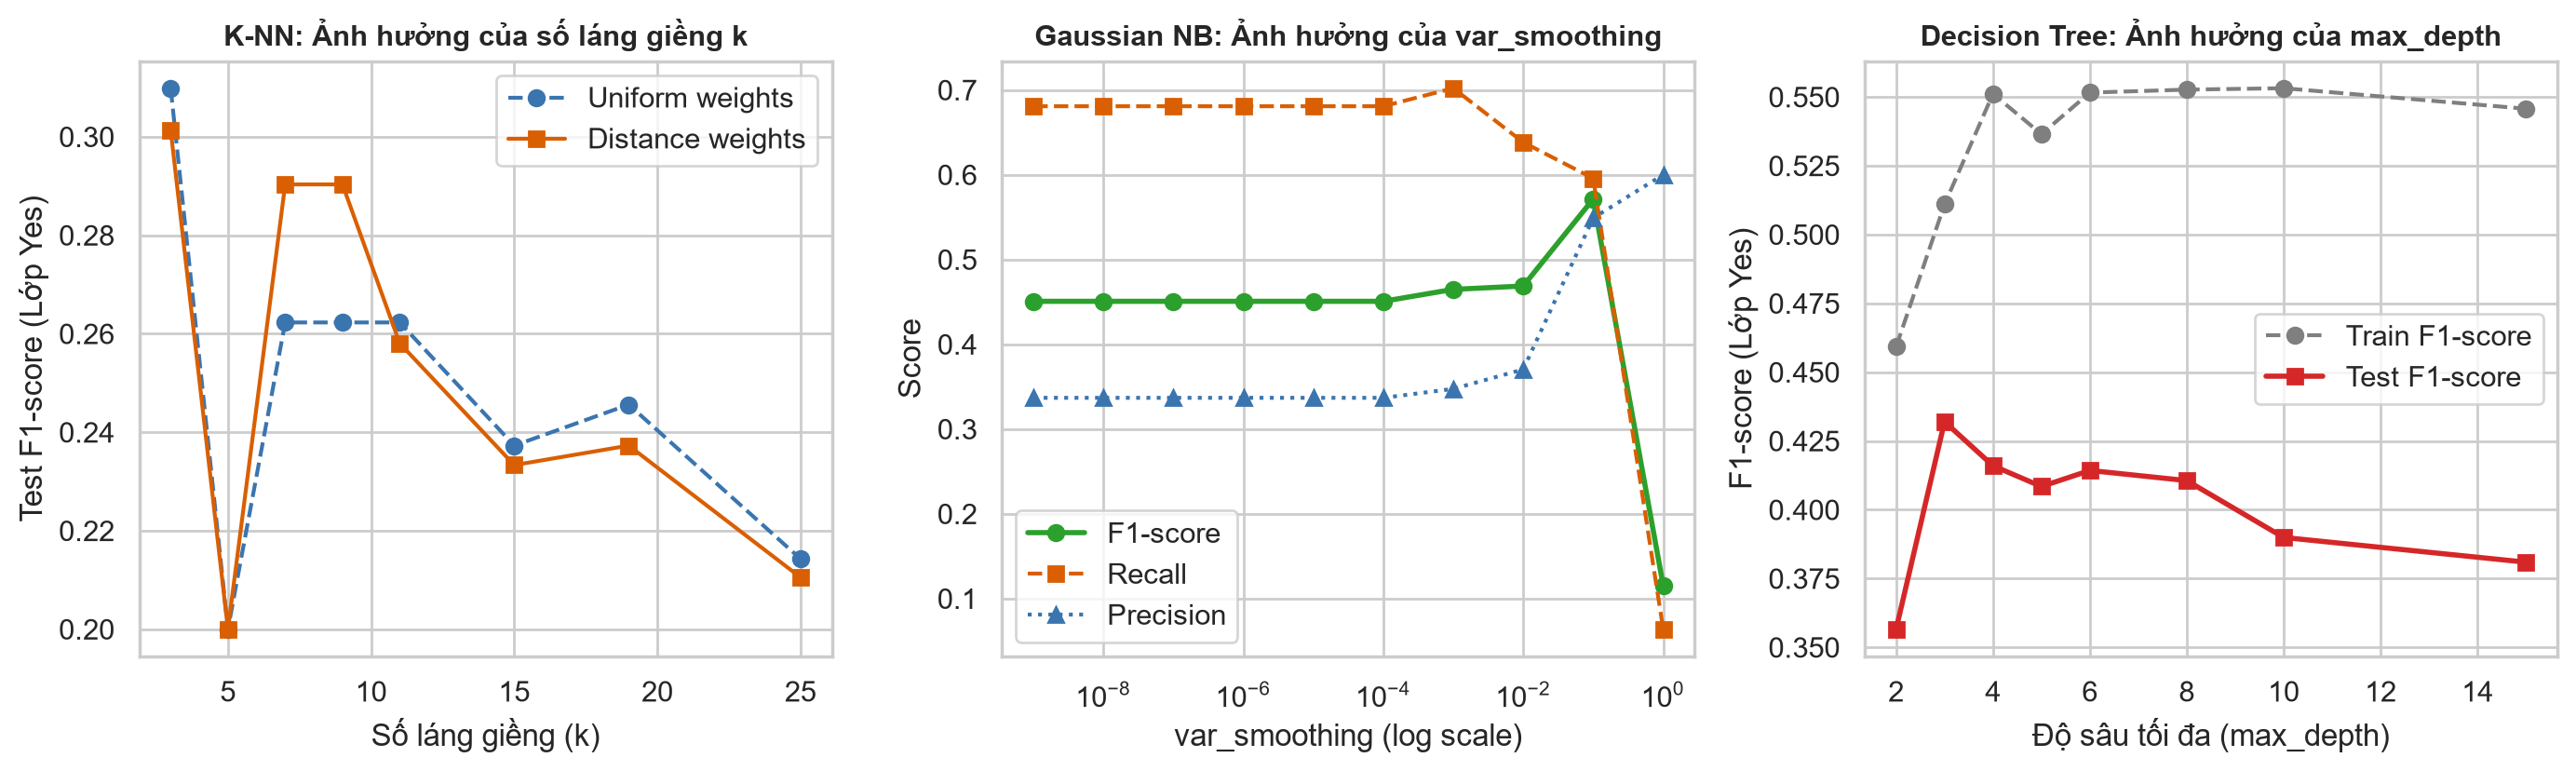
\includegraphics[width=0.98\textwidth]{images/fig5_hyperparameter_tuning.png}
    \caption{Ảnh hưởng của siêu tham số: số láng giềng $k$ (K-NN), var\_smoothing (Gaussian NB) và max\_depth (Decision Tree)}
    \label{fig:hyper_tuning}
    \Nguon{Nhóm thực hiện trích xuất từ dữ liệu thực nghiệm}
\end{figure}

\begin{enumerate}
    \item \textbf{Ảnh hưởng của $k$ và trọng số \textit{weights} trong K-NN (Hình~\ref{fig:hyper_tuning} trái)}: Khi dùng trọng số đồng nhất (\textit{uniform}), chỉ cần $k \ge 9$ thì lớp đa số \textit{No} áp đảo hoàn toàn khiến $\text{F1-score}$ rơi xuống dưới $0.18$. Khi chuyển sang trọng số nghịch đảo khoảng cách (\textit{weights = 'distance'}) và khoảng cách Manhattan, điểm đỉnh đạt được tại $k = 7$ với $\text{F1} = 0.2903$.
    \item \textbf{Ảnh hưởng của \textit{var\_smoothing} trong Gaussian NB (Hình~\ref{fig:hyper_tuning} giữa)}: Khi $\text{var\_smoothing} \in [10^{-9}, 10^{-3}]$, \textit{Recall} giữ ở mức $\approx 68\%$ nhưng \textit{Precision} thấp ($\approx 34\%$) do phương sai nhỏ của các cột nhị phân đẩy xác suất hậu nghiệm lên quá cao. Khi tăng \textit{var\_smoothing} lên $0.1$, đường \textit{Precision} tăng mạnh lên $54.90\%$ trong khi \textit{Recall} vẫn đạt $59.57\%$, tạo ra điểm giao tối ưu giúp \textit{F1-score} đạt cực đại $0.5714$.
    \item \textbf{Ảnh hưởng của \textit{max\_depth} trong Decision Tree (Hình~\ref{fig:hyper_tuning} phải)}: Khi tăng \textit{max\_depth} từ $2$ lên $15$, đường \textit{Train F1} tăng liên tục từ $0.38$ lên trên $0.75$, nhưng đường \textit{Test F1} đạt đỉnh tại $\text{max\_depth} = 4$ ($0.4160$) rồi suy giảm dần về $0.33$ khi cây quá sâu. Đồ thị này minh chứng trực quan hiện tượng \textbf{Overfitting} khi cây quyết định không được cắt tỉa.
\end{enumerate}

\subsection{Phân tích Ma trận nhầm lẫn (Confusion Matrix) và Đường cong ROC}
Hình~\ref{fig:cm} và Hình~\ref{fig:roc} trình bày Ma trận nhầm lẫn và Đường cong ROC của các mô hình tiêu biểu trên tập Kiểm thử ($N_{\text{test}} = 294$).

\begin{figure}[H]
    \centering
    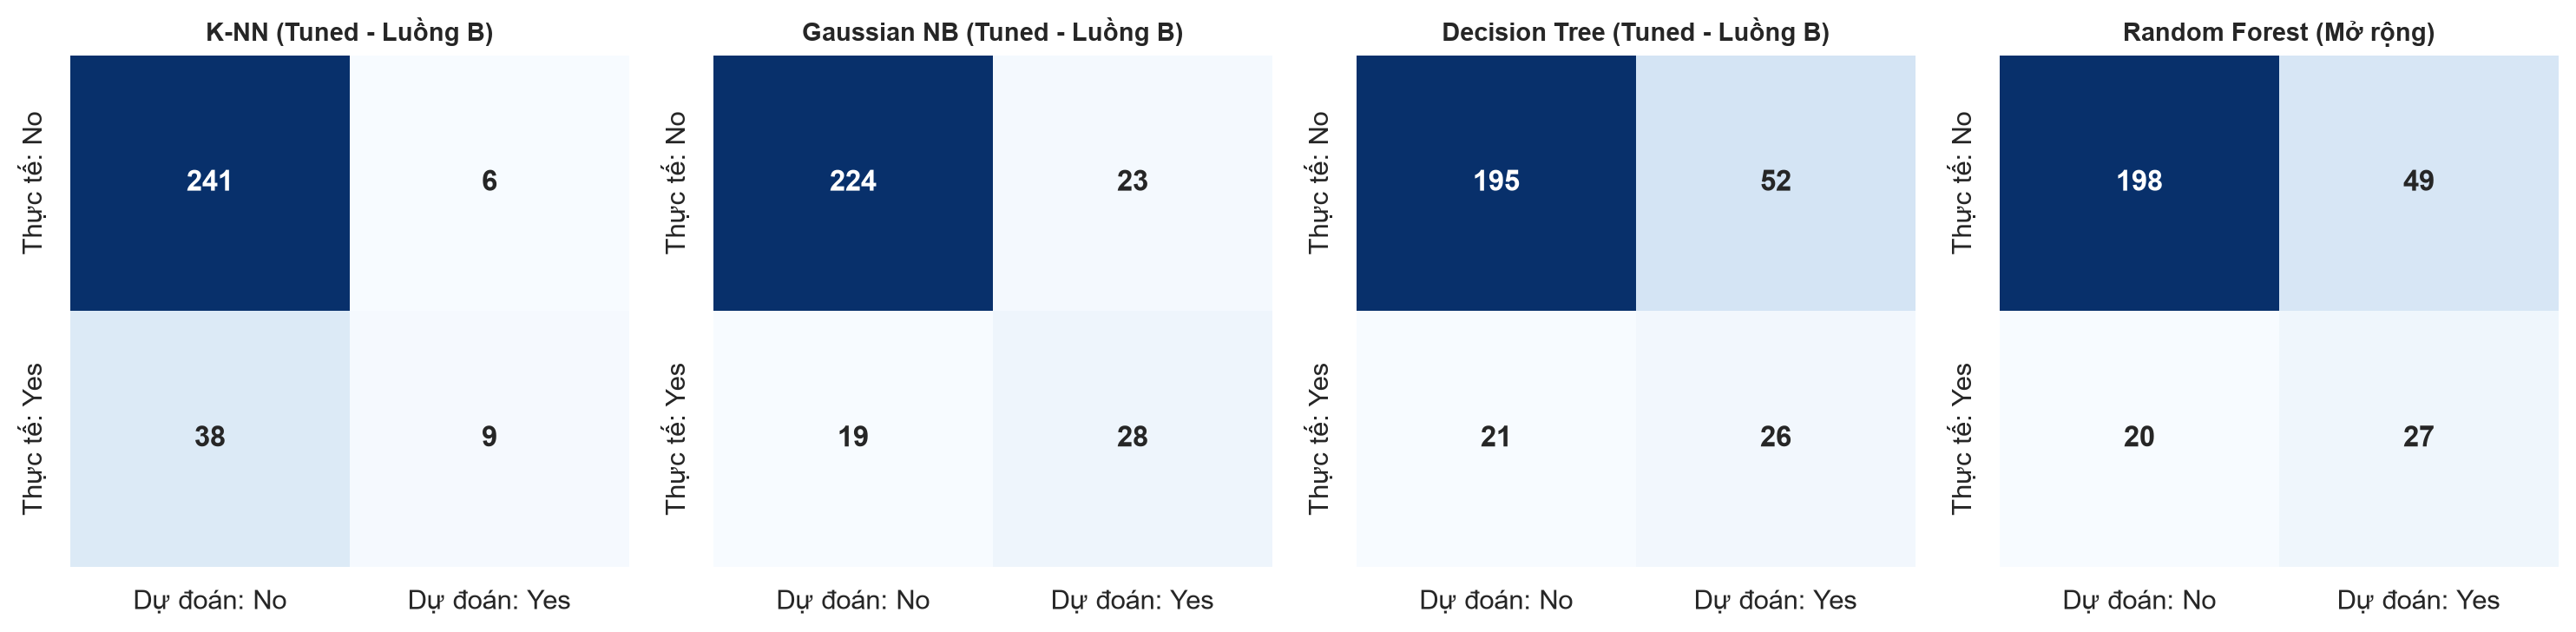
\includegraphics[width=0.98\textwidth]{images/fig7_confusion_matrices.png}
    \caption{Ma trận nhầm lẫn (Confusion Matrix) trên tập Kiểm thử ($N = 294$) của 4 mô hình tiêu biểu}
    \label{fig:cm}
    \Nguon{Nhóm thực hiện trích xuất từ dữ liệu thực nghiệm}
\end{figure}

\begin{figure}[H]
    \centering
    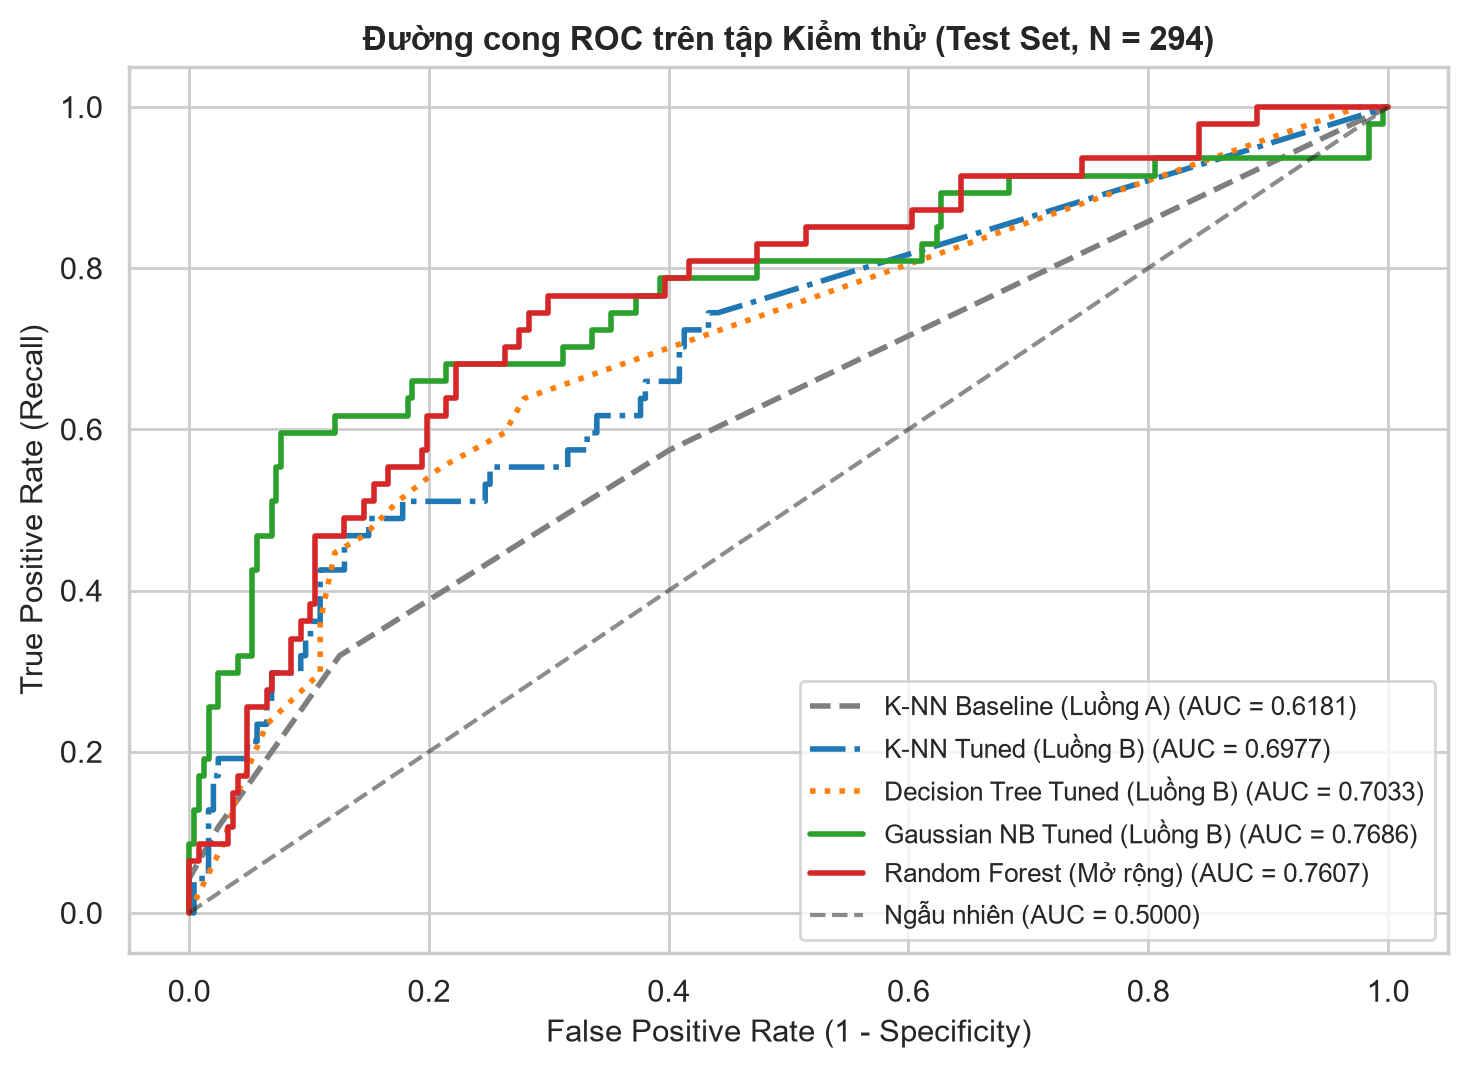
\includegraphics[width=0.76\textwidth]{images/fig8_roc_curves.png}
    \caption{Đường cong ROC so sánh khả năng phân loại trên tập Kiểm thử ($N = 294$)}
    \label{fig:roc}
    \Nguon{Nhóm thực hiện trích xuất từ dữ liệu thực nghiệm}
\end{figure}

Nhìn vào Hình~\ref{fig:cm} và Hình~\ref{fig:roc}, ta thấy sự đối lập thú vị giữa các họ mô hình:
\begin{itemize}
    \item \textbf{K-NN (Tuned -- Luồng B)} rất ``thận trọng'': chỉ dự đoán $15$ người nghỉ việc, trong đó đúng $9$ người ($\text{TP}=9, \text{FP}=6$), đạt $\text{Precision} = 60.0\%$, nhưng bỏ sót tới $\text{FN} = 38/47$ người thực sự nghỉ việc.
    \item \textbf{Gaussian NB (Tuned -- Luồng B)} đạt sự cân bằng tốt nhất: phát hiện đúng $\text{TP} = 28/47$ nhân viên nghỉ việc ($\text{Recall} = 59.57\%$), giữ số lượng báo động giả ở mức thấp ($\text{FP} = 23/247$), đạt $\text{F1} = \mathbf{0.5714}$ và đường cong ROC bao phủ diện tích lớn ($\text{AUC} = 0.7686$).
    \item \textbf{Decision Tree (Tuned -- Luồng B)} và \textbf{Random Forest (Mở rộng)} phát hiện được lần lượt $26/47$ và $27/47$ nhân sự nghỉ việc ($\text{Recall} \approx 55.3\% - 57.5\%$). Đặc biệt, mô hình mở rộng Random Forest cải thiện đáng kể độ mượt của biên quyết định so với cây đơn lẻ, nâng diện tích \textit{ROC-AUC} từ $0.7033$ lên \textbf{0.7607} và \textit{F1-score} lên \textbf{0.4390}.
\end{itemize}

\section{Thảo luận so sánh và phân tích lỗi chuyên sâu}

\subsection{So sánh ưu, nhược điểm của từng thuật toán trong bối cảnh bài toán HR}
Bảng~\ref{tab:so-sanh-thuat-toan} tổng hợp ưu, nhược điểm thực tế của $4$ thuật toán dựa trên bằng chứng thực nghiệm.

\begin{table}[H]
\caption{Tổng hợp so sánh ưu, nhược điểm của các thuật toán trên Đề tài 13}
\label{tab:so-sanh-thuat-toan}
\noindent
\begin{tabularx}{\textwidth}{|L{3.1cm}|Y|Y|}
\hline
\textbf{Thuật toán} & \textbf{Ưu điểm trên bộ dữ liệu HR} & \textbf{Nhược điểm và hạn chế} \\
\hline
\textbf{K-NN} & Đơn giản, không cần giả định phân phối; đạt \textit{Precision} cao ($60.0\%$) khi kết hợp chọn lọc $15$ đặc trưng và khoảng cách Manhattan. & Rất nhạy cảm với mất cân bằng lớp ($84:16$) và không gian hỗn hợp số/nhị phân; \textit{Recall} rất thấp ($19.15\%$), bỏ sót nhiều nhân viên nghỉ việc. \\
\hline
\textbf{Gaussian Naive Bayes} & Huấn luyện cực nhanh; khi kết hợp Luồng B và làm trơn phương sai ($\varepsilon = 0.1$), đạt \textbf{F1 cao nhất ($0.5714$)}, \textbf{Accuracy cao nhất ($85.71\%$)} và \textbf{CV AUC $= 0.8007$}. & Nhạy cảm với đa cộng tuyến nếu dùng dữ liệu thô (Luồng A bị $\text{FP}=99$); giả định phân phối chuẩn cho biến nhị phân chỉ là xấp xỉ. \\
\hline
\textbf{Decision Tree} & Khả năng giải thích (\textit{interpretability}) xuất sắc cho bộ phận HR thông qua các luật \textit{IF-THEN} và độ quan trọng đặc trưng Gini; bắt được $55.3\%$ ca nghỉ việc. & Dễ bị quá khớp (\textit{overfitting}) nếu không giới hạn \textit{max\_depth}; biên quyết định vuông góc từng trục nên độ chính xác xác suất thấp hơn ($\text{AUC}=0.7033$). \\
\hline
\textbf{Random Forest (Mở rộng)} & Giảm mạnh phương sai của Decision Tree đơn lẻ, nâng \textit{CV F1} lên $0.5033$ và \textit{Test AUC} lên $0.7607$; ổn định trước nhiễu. & Khó diễn giải thành một cây quy tắc duy nhất hơn so với Decision Tree đơn lẻ; thời gian tính toán lâu hơn. \\
\hline
\end{tabularx}
\Nguon{Nhóm thực hiện phân tích và đối sánh}
\end{table}

Hình~\ref{fig:feat_imp} minh họa mức độ quan trọng của các đặc trưng (Gini Importance) được trích xuất từ mô hình Cây quyết định trên Luồng B. Kết quả cho thấy đặc trưng tương tác mới \textbf{\textit{OverTime\_Single\_Risk}} đứng vị trí số 1 ($\text{Importance} = 0.250$), tiếp theo là \textbf{\textit{TotalWorkingYears}} ($0.240$), chỉ số hài lòng tổng hợp mới \textbf{\textit{TotalSatisfaction}} ($0.140$) và \textbf{\textit{MonthlyIncome}} ($0.106$). Đây là bằng chứng định lượng rõ ràng giải thích tại sao Luồng B lại vượt trội so với Luồng A.

\begin{figure}[H]
    \centering
    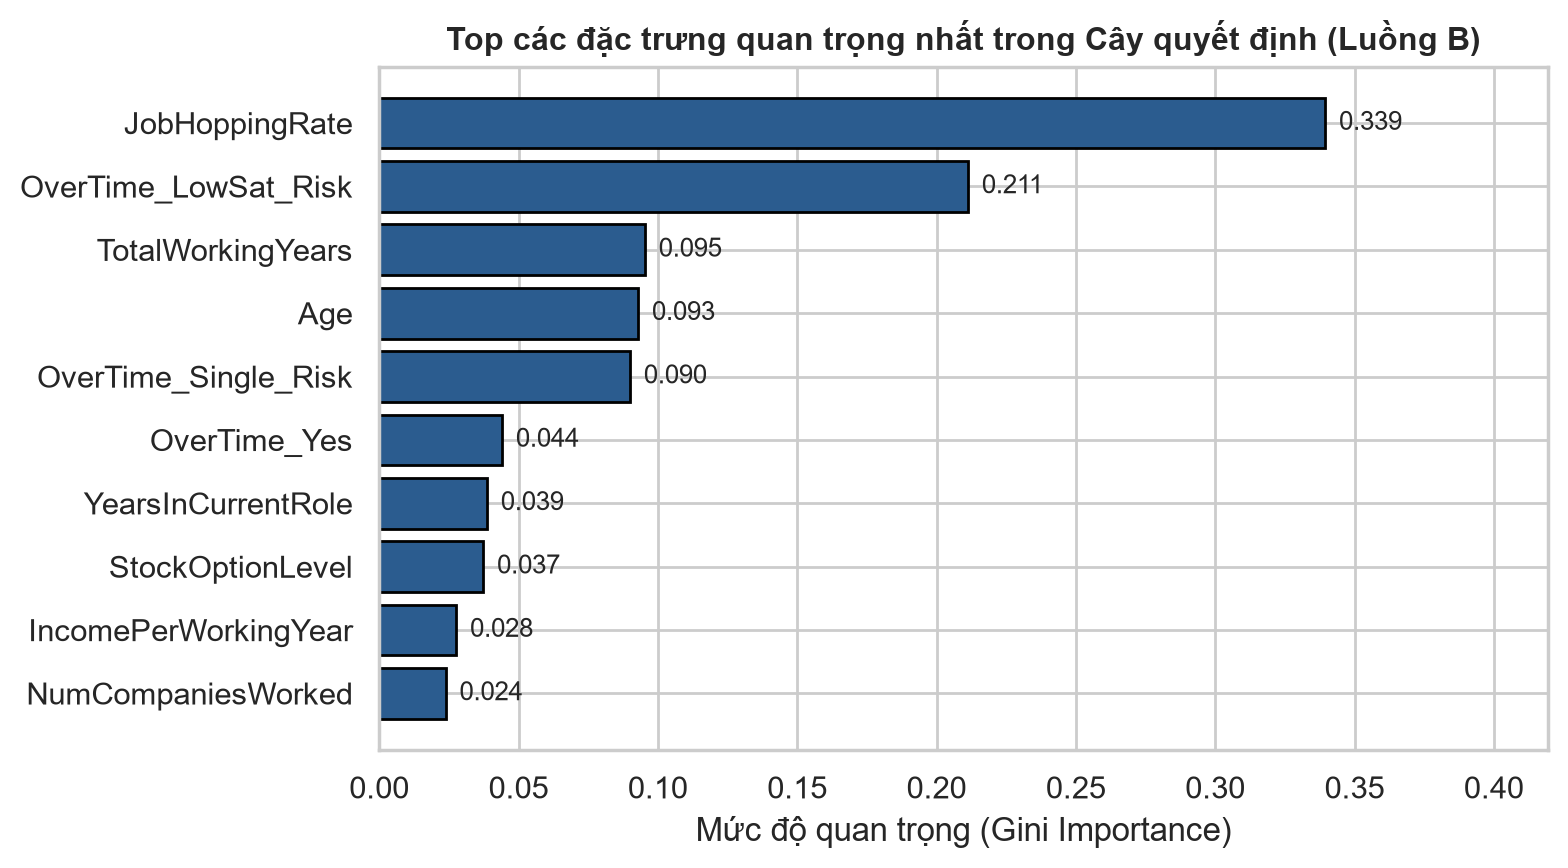
\includegraphics[width=0.80\textwidth]{images/fig9_feature_importance.png}
    \caption{Top các đặc trưng quan trọng nhất (Gini Importance) trong Cây quyết định tại Luồng B}
    \label{fig:feat_imp}
    \Nguon{Nhóm thực hiện trích xuất từ mô hình thực nghiệm}
\end{figure}

\subsection{Phân tích các trường hợp dự đoán sai (Error Analysis: FN và FP)}
Để hiểu rõ tại sao mô hình tốt nhất (\textbf{Gaussian NB Tuned -- Luồng B}) vẫn dự đoán sai $42/294$ mẫu trên tập Test (gồm $\text{FN} = 19$ ca bỏ sót và $\text{FP} = 23$ ca báo động giả), nhóm trích xuất các bản ghi có sai số xác suất lớn nhất từ tệp \textit{error\_analysis\_FN.csv} và \textit{error\_analysis\_FP.csv} tại Bảng~\ref{tab:phan-tich-loi}.

\begin{table}[H]
\caption{Các bản ghi nhân viên bị dự đoán sai điển hình (False Negative và False Positive) trên tập Test}
\label{tab:phan-tich-loi}
\noindent
\setlength{\tabcolsep}{4pt}
\begin{tabularx}{\textwidth}{|c|c|c|Y|r|c|c|c|c|c|c|}
\hline
\textbf{Lỗi} & \textbf{Mã} & \textbf{Tuổi} & \textbf{Vị trí công việc} & \textbf{Lương} & \textbf{OT} & \textbf{Hôn nhân} & \textbf{Cty} & \textbf{Sat} & \textbf{Thực/Đoán} & \textbf{$P(\text{Yes})$} \\
\hline
\textbf{FN} & \#58   & 41 & Research Director   & 19,545 & No  & Married  & 22 & 3 & 1 / 0 & 0.000 \\
\hline
\textbf{FN} & \#165  & 58 & Healthcare Rep.     & 10,312 & No  & Married  & 40 & 4 & 1 / 0 & 0.000 \\
\hline
\textbf{FN} & \#1572 & 53 & Manufacturing Dir.  & 10,169 & No  & Married  & 33 & 4 & 1 / 0 & 0.000 \\
\hline
\textbf{FN} & \#1098 & 44 & Human Resources     & 10,482 & No  & Married  & 20 & 1 & 1 / 0 & 0.001 \\
\hline
\textbf{FP} & \#1839 & 18 & Research Scientist  & 1,514  & No  & Single   & 0  & 3 & 0 / 1 & 0.996 \\
\hline
\textbf{FP} & \#411  & 18 & Sales Rep.          & 1,200  & No  & Single   & 0  & 3 & 0 / 1 & 0.990 \\
\hline
\textbf{FP} & \#1893 & 26 & Research Scientist  & 2,933  & Yes & Married  & 1  & 3 & 0 / 1 & 0.953 \\
\hline
\textbf{FP} & \#22   & 22 & Laboratory Tech.    & 2,935  & Yes & Divorced & 1  & 4 & 0 / 1 & 0.950 \\
\hline
\end{tabularx}
\Nguon{Nhóm thực hiện trích xuất từ outputs/results/error\_analysis\_FN.csv và FP.csv}
\end{table}

Từ Bảng~\ref{tab:phan-tich-loi}, nhóm rút ra các nhận định sâu sắc gắn liền với thực tế quản trị nhân sự:
\begin{enumerate}
    \item \textbf{Nguyên nhân lỗi False Negative (FN -- Bỏ sót người thực sự nghỉ việc)}:
    \begin{itemize}
        \item Nhóm thứ nhất là \textbf{nhân sự cấp cao / thâm niên rất dài}: Ví dụ nhân viên \textit{\#58} (\textit{Research Director}, lương $19,545$ USD, $22$ năm tại công ty, không làm thêm giờ), \textit{\#165} ($58$ tuổi, $40$ năm làm việc, mức hài lòng tuyệt đối $4/4$) và \textit{\#1572} ($53$ tuổi, $33$ năm tại công ty). Mọi đặc trưng của họ đều nằm sâu trong vùng phân phối của lớp ``Ở lại (\textit{No})'' nên mô hình gán xác suất $P(\text{Yes}) \approx 0$. Việc họ rời công ty thực chất đến từ \textbf{yếu tố ngoại sinh} như nghỉ hưu theo tuổi ($58$ tuổi), vấn đề sức khỏe cá nhân hoặc được bổ nhiệm sang vị trí điều hành cấp tập đoàn.
        \item Nhóm thứ hai là \textbf{bất mãn cục bộ bị che lấp bởi lương cao}: Nhân viên \textit{\#1098} có lương cao ($10,482$ USD) và $20$ năm thâm niên nên tổng điểm xác suất thấp, dù điểm hài lòng công việc giảm xuống cực tiểu (\textit{JobSatisfaction = 1}).
    \end{itemize}
    \item \textbf{Ý nghĩa thực tiễn của lỗi False Positive (FP -- Dự đoán nghỉ việc nhưng thực tế đang ở lại)}:
    \begin{itemize}
        \item Các nhân viên \textit{\#1839}, \textit{\#411} ($18$ tuổi, độc thân, mới vào công ty chưa đầy $1$ năm, làm \textit{Sales Representative} hoặc \textit{Research Scientist} với mức lương tối thiểu $1,200 - 1,514$ USD) và \textit{\#1893}, \textit{\#22} (trẻ tuổi, mới làm $1$ năm nhưng đã phải làm thêm giờ \textit{OverTime = Yes}, đi làm xa $16$ dặm) đều có hồ sơ trùng khớp hoàn toàn với nhóm nhân viên dễ nghỉ việc nhất.
        \item Trong bối cảnh ứng dụng thực tế tại doanh nghiệp, $23$ trường hợp FP này \textbf{không phải là sự lãng phí}, mà chính là \textbf{Danh sách nhân sự cần quan tâm sớm (\textit{Proactive Retention Watchlist})}: tại thời điểm chụp cắt ngang dữ liệu họ chưa nộp đơn nghỉ, nhưng xác suất rời bỏ trong $3$--$6$ tháng tới là rất cao nếu phòng HR không kịp thời hỗ trợ lộ trình hội nhập hoặc điều chỉnh khối lượng tăng ca.
    \end{itemize}
\end{enumerate}

\subsection{Hạn chế của dữ liệu và của giải pháp hiện tại}
\begin{itemize}
    \item \textbf{Hạn chế về tính chất dữ liệu tĩnh (\textit{Cross-sectional Data})}: Bộ dữ liệu chỉ phản ánh trạng thái tại một thời điểm duy nhất, thiếu thông tin chuỗi thời gian (\textit{time-series}) như xu hướng giảm điểm hài lòng qua các kỳ đánh giá hoặc sự gia tăng đột biến số giờ tăng ca trong quý gần nhất.
    \item \textbf{Gộp chung nhiều lý do nghỉ việc vào cùng một nhãn \textit{Yes}}: Dữ liệu không tách biệt giữa nghỉ việc tự nguyện do bất mãn (\textit{voluntary turnover}) với nghỉ hưu theo chế độ (\textit{retirement}) ở nhóm $55$--$60$ tuổi, tạo ra các điểm nhiễu nhãn làm giảm trần \textit{Recall} của mọi thuật toán.
\end{itemize}


% =========================
% PHẦN CUỐI BÁO CÁO
% =========================
\clearpage
\UnnumberedChapter{KẾT LUẬN VÀ HƯỚNG PHÁT TRIỂN}

\section*{1. Tóm tắt các kết quả chính đạt được}
Qua quá trình thực hiện bài tập lớn học phần \textbf{Nhập môn Học máy (FIT4013)} với \textbf{Đề tài 13: Dự đoán nhân viên có khả năng nghỉ việc}, nhóm đã hoàn thành toàn bộ các mục tiêu đề ra về mặt kiến thức và kỹ năng:
\begin{itemize}
    \item \textbf{Khám phá dữ liệu (EDA) toàn diện}: Đã phân tích sâu cấu trúc $1,470$ mẫu $\times 35$ thuộc tính của bộ dữ liệu IBM HR Analytics, chỉ ra tỷ lệ mất cân bằng lớp $83.88\% : 16.12\%$, nhận diện $4$ cột hằng số/định danh cần loại bỏ, $3$ cột tỷ lệ lương ngẫu nhiên gây nhiễu khoảng cách và các cặp biến đa cộng tuyến mạnh ($r = 0.95$).
    \item \textbf{Chứng minh hiệu quả của Pipeline cải tiến (Luồng B)}: Việc thiết kế bộ biến đổi \textit{HRFeatureEngineer} tạo ra $8$ đặc trưng nghiệp vụ nhân sự mới (đặc biệt là \textit{OverTime\_Single\_Risk}, \textit{OverTime\_LowSat\_Risk}, \textit{TotalSatisfaction}), kết hợp chuẩn hóa kháng ngoại lệ \textit{RobustScaler} và lọc đặc trưng \textit{SelectKBest}, đã giúp cải thiện hiệu năng trên toàn bộ các thuật toán so với Luồng A (Pipeline cơ bản):
    \begin{itemize}
        \item \textbf{K-Nearest Neighbors (Tuned)}: \textit{F1-score} tăng từ $0.1132$ lên \textbf{0.2903} (\textbf{+156.4\%}), \textit{Precision} đạt \textbf{60.00\%}.
        \item \textbf{Decision Tree (Tuned)}: \textit{F1-score} tăng từ $0.3529$ lên \textbf{0.4160} (\textbf{+17.9\%}), \textit{Recall} đạt \textbf{55.32\%}.
        \item \textbf{Gaussian Naive Bayes (Tuned, $\varepsilon = 0.1$)}: Đạt hiệu năng xuất sắc nhất toàn bộ thực nghiệm với \textbf{\textit{F1-score} $= 0.5714$} (\textbf{+36.5\%} so với Luồng A), \textbf{\textit{Accuracy} $= 85.71\%$}, \textbf{\textit{Recall} $= 59.57\%$}, \textbf{\textit{Precision} $= 54.90\%$} và \textbf{\textit{CV ROC-AUC} $= 0.8007$}.
    \end{itemize}
    \item \textbf{Hoàn thiện kỹ thuật mở rộng và ứng dụng thực tiễn}: Nhóm đã triển khai thêm mô hình học kết hợp \textbf{Random Forest Ensemble} ($\text{Test AUC} = 0.7607$) và xây dựng ứng dụng \textbf{Web App Demo (\textit{app.py})} hỗ trợ bộ phận Nhân sự dự đoán trực quan nguy cơ nghỉ việc và đề xuất giải pháp giữ chân nhân viên theo thời gian thực.
\end{itemize}

\section*{2. Khuyến nghị ứng dụng cho quản trị nhân sự và hướng phát triển}
\begin{enumerate}
    \item \textbf{Khuyến nghị chính sách quản trị nhân sự từ kết quả mô hình}:
    \begin{itemize}
        \item \textit{Kiểm soát khối lượng làm thêm giờ (\textit{OverTime})}: Nhóm nhân viên làm thêm giờ có tỷ lệ nghỉ việc cao gấp $3$ lần ($30.53\%$ so với $10.44\%$). Doanh nghiệp cần giới hạn trần tăng ca liên tiếp và bổ sung cơ chế nghỉ bù hoặc phụ cấp thỏa đáng, đặc biệt ở bộ phận \textit{Sales Representative} và \textit{Laboratory Technician}.
        \item \textit{Chăm sóc nhóm nhân sự trẻ trong 2 năm đầu (\textit{NewHireRisk})}: Tổ chức các buổi trao đổi định kỳ 1-1 (\textit{Stay Interview}) cho các nhân viên dưới $25$ tuổi, độc thân, mới gia nhập công ty dưới $2$ năm có điểm hài lòng môi trường làm việc $\le 2$.
    \end{itemize}
    \item \textbf{Hướng phát triển kỹ thuật trong tương lai}:
    \begin{itemize}
        \item \textit{Tinh chỉnh ngưỡng xác suất theo chi phí (\textit{Cost-sensitive Thresholding})}: Hạ ngưỡng phân lớp từ $\tau = 0.50$ xuống $\tau = 0.35$ khi doanh nghiệp muốn ưu tiên tối đa hóa \textit{Recall} (bắt được $>75\%$ nhân sự có ý định nghỉ việc).
        \item \textit{Kết hợp lấy mẫu cân bằng SMOTE/ENN bên trong Pipeline}: Thử nghiệm \textit{SMOTE-ENN} riêng cho K-NN để cải thiện mật độ láng giềng lớp thiểu số.
        \item \textit{Tích hợp SHAP Values}: Hiển thị mức đóng góp cụ thể của từng yếu tố lên quyết định dự đoán của từng cá nhân trên giao diện Web App Demo.
    \end{itemize}
\end{enumerate}


\clearpage
\appendix
\UnnumberedChapter{PHỤ LỤC}

\section*{Phụ lục 1. Hướng dẫn chạy chương trình và tái lập kết quả}
Để tái tạo toàn bộ kết quả thực nghiệm, biểu đồ và chạy thử nghiệm ứng dụng Web App Demo của nhóm, giảng viên và người đọc có thể thực hiện theo $3$ bước sau tại thư mục gốc của dự án:
\begin{enumerate}
    \item \textbf{Cài đặt các thư viện phụ thuộc}:
    \begin{lstlisting}[language=bash]
pip install -r requirements.txt
    \end{lstlisting}
    \item \textbf{Chạy kịch bản tái lập toàn bộ Pipeline (Luồng A, Luồng B, 9 biểu đồ và lưu mô hình)}:
    \begin{lstlisting}[language=bash]
python run_experiments.py
    \end{lstlisting}
    \item \textbf{Khởi chạy ứng dụng Web App Demo dự đoán nghỉ việc tương tác}:
    \begin{lstlisting}[language=bash]
python app.py
# Sau do mo trinh duyet truy cap: http://127.0.0.1:5000
    \end{lstlisting}
\end{enumerate}


\clearpage
\UnnumberedChapter{DANH MỤC TÀI LIỆU THAM KHẢO}

\section*{Tiếng Việt}

\begin{enumerate}[label={[\arabic*]}]
    \item Lê Thị Thùy Trang. (2026). \textit{Hướng dẫn thực hiện Bài tập lớn Học phần Nhập môn Học máy (FIT4013)}. Khoa Công nghệ thông tin, Trường Đại học Đại Nam, Hà Nội.
    \item Vũ Hữu Tiệp. (2020). \textit{Machine Learning cơ bản}. Nhà xuất bản Khoa học và Kỹ thuật, Hà Nội.
\end{enumerate}

\section*{Tiếng Anh}

\begin{enumerate}[label={[\arabic*]}, resume]
    \item James, G., Witten, D., Hastie, T., \& Tibshirani, R. (2021). \textit{An Introduction to Statistical Learning: with Applications in R / Python} (2nd ed.). Springer.
    \item Pedregosa, F., Varoquaux, G., Gramfort, A., Michel, V., Thirion, B., Grisel, O., \ldots \& Duchesnay, E. (2011). Scikit-learn: Machine Learning in Python. \textit{Journal of Machine Learning Research}, 12, 2825--2830.
    \item IBM Watson Analytics. (2017). \textit{IBM HR Analytics Employee Attrition \& Performance Dataset}. Kaggle / IBM Sample Data Sets.
\end{enumerate}


\end{document}
